%%-----------------------------------------------------------------------------
%%                           DOCUMENT INFO
%%
%%-----------------------------------------------------------------------------
\documentclass[12pt,compress,handout]{beamer}  %For printable version
%\documentclass[12pt,compress]{beamer}         %For presentation version

%% -------------- Packages ------------------------------
\usepackage{amssymb}
\usepackage{amsmath}
\usepackage{amsthm}
\usepackage{colortbl}
\usepackage{graphicx}
\usepackage{hyperref}
\usepackage[sort]{natbib}
\usepackage{rotating}
\usepackage{subfigure}
\usepackage{multirow}
\usepackage{tikz}
\usetikzlibrary{shapes,arrows,trees,snakes,positioning,fit,shadows}     % library for tikz
\usepackage{bm}
\usepackage{epstopdf}
\usepackage{setspace}
\usepackage{bigstrut}
\usepackage{caption}
\usepackage{longtable}
\usepackage{lscape}
\usepackage{epstopdf}
\usepackage{multirow}
\usepackage{enumerate}
\usepackage{csquotes}
\usepackage{pdfpages}
\usepackage{float}
\usepackage{booktabs}

%% ----- Theme and formatting for printable version ---------
\mode<handout>{
  \useoutertheme{split}
  \useinnertheme{rounded}
  \usecolortheme{seahorse}
  \usecolortheme{rose}
  %\setbeamertemplate{footline}[frame number]
  \usepackage{pgfpages}
  %\pgfpagesuselayout{resize to}[letterpaper,landscape]

  \setbeamertemplate{footline}
{
 \leavevmode%
 \hbox{%
 \begin{beamercolorbox}[wd=.3\paperwidth,ht=2.25ex,dp=1ex,center]{author in head/foot}%
   \usebeamerfont{author in head/foot}\insertshortauthor~~%\beamer@ifempty{\insertshortinstitute}{}{(\insertshortinstitute)
 \end{beamercolorbox}%
 \begin{beamercolorbox}[wd=.6\paperwidth,ht=2.25ex,dp=1ex,center]{title in head/foot}%
   \usebeamerfont{title in head/foot}\insertshorttitle
 \end{beamercolorbox}%
 \begin{beamercolorbox}[wd=.1\paperwidth,ht=2.25ex,dp=1ex,right]{date in head/foot}%
   %\usebeamerfont{date in head/foot}\insertshortdate{}\hspace*{2em}
   \insertframenumber{} / \inserttotalframenumber\hspace*{2ex}
 \end{beamercolorbox}}%
 \vskip0pt%
}
}

%% ----- Theme for projector DYNAMIC display version --------------
\mode<beamer>{
  \useoutertheme{shadow}
  \usecolortheme{whale}
  \usecolortheme{orchid}
  \useinnertheme[shadow=true]{rounded}
  \setbeamerfont{block title}{size={}}
  \hypersetup{pdfpagemode=FullScreen}

  \setbeamertemplate{footline}
{
 \leavevmode%
 \hbox{%
 \begin{beamercolorbox}[wd=.5\paperwidth,ht=2.25ex,dp=1ex,center]{author in head/foot}%
   \usebeamerfont{author in head/foot}\insertshortauthor~~%\beamer@ifempty{\insertshortinstitute}{}{(\insertshortinstitute)
 \end{beamercolorbox}%
 \begin{beamercolorbox}[wd=.5\paperwidth,ht=2.25ex,dp=1ex,center]{title in head/foot}%
   \usebeamerfont{title in head/foot}\insertshorttitle
 \end{beamercolorbox}%
 }%
 \vskip0pt%
}
}

%% ----- Formatting for beamer ----------------------------
\mode<handout>{
\setbeamertemplate{headline}
{
  \leavevmode%
  \hbox{%
    \begin{beamercolorbox}[wd=\paperwidth,ht=2.25ex,dp=1ex,center]{section in head/foot}%
      \insertsectionnavigationhorizontal{\paperwidth}{}{}%
     \end{beamercolorbox}}
  \vskip0pt%
}
}

\mode<beamer>{
\setbeamertemplate{headline}
{
  \leavevmode%
  \hbox{%
    \begin{beamercolorbox}[wd=\paperwidth,ht=2.25ex,dp=1ex,center]{section in head/foot}%
      \insertsectionnavigationhorizontal{\paperwidth}{}{}%
     \end{beamercolorbox}}
  \vskip2pt%
}
}

\setbeamertemplate{mini frames}[default]%
\setbeamertemplate{sections/subsections in toc}[ball]%
\setbeamertemplate{mini frame in other subsection}[default][0]%
\setbeamertemplate{frametitle continuation}[from second]%
\setbeamersize{text margin left=0.2 in}%
\setbeamersize{text margin right=0.2 in}%
\setbeamerfont{frametitle}{size=\small}%
\setbeamerfont{infolines}{size=\footnotesize}%

%% ----- The next 3 lines allow natbib to work properly in a Beamer Document --
\makeatletter
\def\newblock{\beamer@[EMAIL PROTECTED]}
\makeatother

%%----- User-defined LaTeX commands (cruft from numerous older versions) ------

\newcommand{\orth}{\ensuremath{\perp\!\!\!\perp}}%

\DeclareMathAlphabet{\mathitbf}{OML}{cmm}{b}{it}

\renewcommand{\figurename}{Figure~\arabic{figure}}
\renewcommand{\tablename}{Table~\arabic{table}}


%%%%%%%%%%%%%%%%%%%%%%%%%%%%%%%%%%%%%%%%%%%%%%%%%%%%%%%%%%%%%%%%%%%%%%%%%%%%%%
\begin{document}


%%%%%%%%%%%%%%%%%%%%%%%%%%%%%%%%%%%%%%%%%%%%%%%%%%%%%%%%%%%%%%%%%%%%%%%%%%%%%%%
\title{Ben-Porath Notes}

\author{James Heckman\\University of Chicago}

\date{Econ 350\\
This draft, \today}


%%%%%%%%%%%%%%%%%%%%%%%%%%%%%%%%%%%%%%%%%%%%%%%%%%%%%%%%%%%%%%%%%%%%%%%%%%%%%%%
\frame{\titlepage}


%%%%%%%%%%%%%%%%%%%%%%%%%%%%%%%%%%%%%%%%%%%%%%%%%%%%%%%%%%%%%%%%%%%%%%%%%%%%%%%
\section[Human Capital]{Notes on Ben-Porath Human Capital Model}


%%%%%%%%%%%%%%%%%%%%%%%%%%%%%%%%%%%%%%%%%%%%%%%%%%%%%%%%%%%%%%%%%%%%%%%%%%%%%%%
\begin{frame}
\begin{center}
\textbf{\insertsection}
\end{center}
\begin{itemize}[<+->]
\item Perfect Capital Markets

\item No Nonmarket Benefits of Human Capital

\item Fixed Labor Supply

\item $H$ is human capital

\item $I \in [0,1]$ is investment time

\item $D$ is goods input

\item $F$ is a strictly concave function in two normal inputs
\end{itemize}
\end{frame}


%%%%%%%%%%%%%%%%%%%%%%%%%%%%%%%%%%%%%%%%%%%%%%%%%%%%%%%%%%%%%%%%%%%%%%%%%%%%%%%
\begin{frame}
\frametitle{Human Capital Production Function}

\begin{itemize}[<+->]
\item $\dot{H}(t) = F(I(t),H(t),D(t)) - \sigma H(t)$

\item $F(I(t),H(t),D(t))=F(I(t)H(t),D(t)) \quad$ (neutrality)

\item $R$ is rental rate of human capital.

\item Potential earnings: $Y(t) = RH(t)$.

\item Observed earnings:
\begin{equation*}
E(t) = RH(t) - \underset{\begin{array}{c}\text{earnings}\\
\text{foregone}\end{array}}{\underbrace{RI(t)H(t)}} -
\underset{\begin{array}{c}\text{direct goods}\\
\text{costs}\end{array}}{\underbrace{P_{D}D(t)}}
\end{equation*}
\end{itemize}
\end{frame}


%%%%%%%%%%%%%%%%%%%%%%%%%%%%%%%%%%%%%%%%%%%%%%%%%%%%%%%%%%%%%%%%%%%%%%%%%%%%%%%
\begin{frame}
\begin{itemize}[<+->]
\item Consumer problem (max with respect to $I(t), D(t)$):
\begin{equation*}
\int\limits_{0}^{T}e^{-rt}E(t)dt\qquad \text{given } H(0) = H_{0}
\end{equation*}

\item Formal solution (Hamiltonian): Flow of value from the optimal lifetime
program
\begin{equation*}
\underset{\text{current
flow}}{\underbrace{e^{-rt}[RH(t)-RI(t)H(t)-P_{D}D(t)]}}\underset{\text{of human
capital}}{\underset{\text{shadow price}}{+\underbrace{\mu (t)}[\dot{H}]}}
\end{equation*}

\end{itemize}
\end{frame}


%%%%%%%%%%%%%%%%%%%%%%%%%%%%%%%%%%%%%%%%%%%%%%%%%%%%%%%%%%%%%%%%%%%%%%%%%%%%%%%
\begin{frame}
\begin{itemize}[<+->]
\item FOC Conditions (for interior solution):
\begin{gather*}
I(t): \quad R e^{-rt}H(t)=\mu (t)F_{1}H(t)\\
\\
D(t): \quad e^{-rt}P_{D}=\mu (t)F_{2}\\
\\
\dot{\mu}(t)=-e^{-rt}[R-RI(t)]-\mu (t)F_{1}I(t)+\mu (t)\sigma
\end{gather*}
\end{itemize}
\end{frame}


%%%%%%%%%%%%%%%%%%%%%%%%%%%%%%%%%%%%%%%%%%%%%%%%%%%%%%%%%%%%%%%%%%%%%%%%%%%%%%%
\begin{frame}
\begin{itemize}[<+->]
\item Use FOC for investment to obtain:
\begin{equation*}
\dot{\mu}(t)=-e^{-rt}R+\mu (t)\sigma .
\end{equation*}
Define $g(t)=\mu(t)e^{+rt}$\\\vspace{.2in}
$\dot{g}(t)=\dot{\mu}e^{+rt}+r\mu(t)e^{+rt}$\\\vspace{.2in}
$\dot{g}(t)=(\sigma+r)g(t)-R.$
\end{itemize}
\end{frame}


%%%%%%%%%%%%%%%%%%%%%%%%%%%%%%%%%%%%%%%%%%%%%%%%%%%%%%%%%%%%%%%%%%%%%%%%%%%%%%%
\begin{frame}
\begin{itemize}[<+->]
\item
Transversality: $\lim_{t\rightarrow T}\mu (t)H(t)=0$
\begin{gather*}
\therefore \mu (T)=0\Longrightarrow g(T)=0\\
\\
 g(t)=\dfrac{R\left(
1-e^{(\sigma+r)(t-T)}\right) }{\sigma +r}.
\end{gather*}

\item Note that g(t) is a discount factor that adjusts for exponential
depreciation of gross investment.

\item
$\dot{H}(t) + \sigma H(t) = F(IH(t),D(t))$.
\end{itemize}
\end{frame}


%%%%%%%%%%%%%%%%%%%%%%%%%%%%%%%%%%%%%%%%%%%%%%%%%%%%%%%%%%%%%%%%%%%%%%%%%%%%%%%
\begin{frame}

\begin{itemize}[<+->]
\item
$0 < I(t) < 1$, we can set up the problem in a ``myopic''
way.\medskip

\item
Gross ``output'' is $F(I(t)H(t),D(t))$.\medskip

\item
Returns on gross output: $g(t)$.\medskip

\item
Costs: $P_{D}D(t) + RI(t)H(t)$.\medskip

\item
Note: these are costs and returns as of period $t$.
\end{itemize}
\end{frame}


%%%%%%%%%%%%%%%%%%%%%%%%%%%%%%%%%%%%%%%%%%%%%%%%%%%%%%%%%%%%%%%%%%%%%%%%%%%%%%%
\begin{frame}

\small

\begin{itemize}[<+->]
\item
The agent's problem is:
\begin{equation*}
    \max_{I(t),D(t)}\left[  g(t) F(I(t)H(t),D(t)) - P_{D}D(t)
    - RI(t)H(t)=0\right]
\end{equation*}
\end{itemize}

FOC:
\begin{itemize}
\item
$g(t)F_{1}(I(t)H(t),D(t))H(t)=RH(t)$

\item
$g(t)F_{2}(I(t)H(t),D(t)) -P_{D}=0$.
\end{itemize}

Demand functions are inverted first order conditions:

\begin{itemize}[<+->]
\item
$I(t)H(t)=I(t)H\left( \dfrac{R}{g(t)},\dfrac{P_{D}}{g(t)}\right)$

\item
$D(t)=D\left( \dfrac{R}{g(t)},\dfrac{P_{D}}{g(t)}\right)$
\end{itemize}

From normality of inputs, since $\dot{g}(t)<0$, we have:

\begin{itemize}
\item $\dot{IH}(t)<0$, $\dot{D}(t)<0$.
\end{itemize}
\end{frame}


%%%%%%%%%%%%%%%%%%%%%%%%%%%%%%%%%%%%%%%%%%%%%%%%%%%%%%%%%%%%%%%%%%%%%%%%%%%%%%%
\begin{frame}
\begin{itemize}[<+->]
\item
Then, if $\sigma =0$, $\dot{E}=RF(I(t)H(t),D(t))-R\,\dot{IH}(t)
-P_{D}\dot{D}(t)>0$.\medskip

\item
Otherwise earnings can rise and then fall over the life cycle.
($\sigma \neq 0$).\medskip

\item
What about $\ddot{E}(t)$? Ben Porath chose a Cobb-Douglas form for
$F(I(t)H(t),D(t))$ and proves $\ddot{E}(t) < 0$.\medskip

\item
$\therefore $\ Earnings increase at a
decreasing rate over the life cycle.\medskip

\item
To simplify derivations, let $F_{2} \equiv 0$ (i.e.\ ignore $D(t)$).
\end{itemize}
\end{frame}


%%%%%%%%%%%%%%%%%%%%%%%%%%%%%%%%%%%%%%%%%%%%%%%%%%%%%%%%%%%%%%%%%%%%%%%%%%%%%%%
\begin{frame}
\begin{itemize}[<+->]
\item
First order condition for investment is:\\\vspace{.2in}
$g(t)F^{\prime }(IH)=R.$\\\vspace{.1in} $\dot{g}=(\sigma \
+r)g(t)-R$\\\vspace{.2in}

\item
Differentiate the first order condition for investment.

\item
Set $R = 1$ (for convenience)\\\vspace{.2in} (Note that
$\dfrac{\dot{g}}{g}=\sigma +r-\dfrac{1}{g})$\\\vspace{.2in}
$\dot{g}(t)F^{\prime }(I(t)H(t))+g(t)F^{\prime \prime
}(I(t)H(t))\dot{I(t)H(t)}=0$.\\\vspace{.2in}
Thus\qquad $\dot{IH(t)}=-\left( \dfrac{\dot{g}(t)}{g(t)}\right) \left[ \dfrac{%
F^{\prime }}{F^{\prime \prime }}\right] .$
\end{itemize}
\end{frame}


%%%%%%%%%%%%%%%%%%%%%%%%%%%%%%%%%%%%%%%%%%%%%%%%%%%%%%%%%%%%%%%%%%%%%%%%%%%%%%%
\begin{frame}
\begin{itemize}[<+->]
\item To simplify notation, drop ``t'' argument for $I(t),H(t),g(t)$ unless it
clarifies matters to keep it explicit
\item Then $\ddot{IH}=-\left[ \dfrac{\ddot{g}}{g}-\left( \dfrac{\dot{g
}}{g}\right) ^{2}\right] \dfrac{F^{\prime }}{F^{\prime \prime }}$
$-\dfrac{\dot{g}}{g}\left[ \dot{IH}-\dfrac{ F^{\prime }F^{\prime
\prime \prime }}{(F^{\prime \prime })^{2}}\dot{IH} \right] .$
\item Note that $\ddot{g} = (\sigma + r)\dot{g}$.
\item $\therefore $\ $\dfrac{\ddot{g}}{\dot{g}}=(\sigma +r)$\ and $\dfrac{\ddot{g}}{g}=(\sigma +r)\dfrac{\dot{g}}{g}$ ($\dot{g} \neq 0$).
\item Thus, substituting for $\dot{IH}$ we have\\\vspace{.2in} $\ddot{IH}=-\left[
\dfrac{\text{\"{g}}}{\text{g}}-\left( \dfrac{\dot{g}}{g}\right) ^{2}\right] \dfrac{F^{\prime }}{F^{\prime \prime }}+\left( \dfrac{%
\dot{g}}{g}\right) ^{2}\left[ 1-\dfrac{F^{\prime }F^{\prime \prime \prime }}{%
(F^{\prime \prime })^{2}}\right] \left[ \dfrac{F^{\prime
}}{F^{\prime \prime }}\right] .$
\end{itemize}
\end{frame}


%%%%%%%%%%%%%%%%%%%%%%%%%%%%%%%%%%%%%%%%%%%%%%%%%%%%%%%%%%%%%%%%%%%%%%%%%%%%%%%
\begin{frame}
\begin{itemize}[<+->]
\item Earnings growth is given by (recall $R = 1$)
\item $\dot{E}=F(IH)-\dot{IH}- \sigma H$\\
\item $\ddot{E}=F^{\prime }(IH)\dot{IH}-\ddot{IH}-\sigma \dot{H}$\\
\item Since $F^{\prime }\ $= $\dfrac{\text{1}}{\text{g}}$\ we have that\\
$\ddot{E} = \dfrac{1}{g}\dot{IH} - \ddot{IH} - \sigma \dot{H}$\\
\item Set $\sigma =0$ for the moment and use the expression for
$\dot{IH}$ given above (including $\dot{IH}$).
\end{itemize}
\end{frame}


%%%%%%%%%%%%%%%%%%%%%%%%%%%%%%%%%%%%%%%%%%%%%%%%%%%%%%%%%%%%%%%%%%%%%%%%%%%%%%%
\begin{frame}

Thus
\begin{itemize}[<+->]
\item $\ddot{E}= \dot{IH}\left[ \dfrac{1}{g}+\dfrac{\dot{g}}{g}\left(1-
\dfrac{F^{\prime }F^{\prime \prime \prime }}{(F^{\prime \prime })^{%
\text{2}}}\right)\right] $+$\left( \dfrac{\ddot{g}}{g}-\left( \dfrac{\dot{g}}{g}%
\right) ^{2}\right) \dfrac{F^{\prime }}{F^{\prime \prime }}.$\vspace{.3in}
\item Use
$\dot{IH} = -\dfrac{\dot{g}}{g}\dfrac{F^{\prime }}{F^{\prime \prime }}$ and $\dfrac{%
\ddot{g}}{g}\ =(\sigma \ +r)\dfrac{\dot{g}}{g}$ to conclude that
\end{itemize}
\end{frame}


%%%%%%%%%%%%%%%%%%%%%%%%%%%%%%%%%%%%%%%%%%%%%%%%%%%%%%%%%%%%%%%%%%%%%%%%%%%%%%%
\begin{frame}
\begin{eqnarray*}
\text{\"{E}} &=&-\frac{\text{\.{g}}}{\text{g}}\left[ \frac{\text{F}%
^{\prime }}{\text{F}^{\prime \prime }}\right] \left\{ \frac{\text{1}}{\text{g%
}}+\frac{\text{\.{g}}}{\text{g}}\left( \text{1}-\frac{\text{F}^{\prime }%
\text{F}^{\prime \prime }}{\text{(F}^{\prime \prime }\text{)}^{\text{2}}}%
\right) \right\} \\
&&+\left( (\sigma \text{ + r)}\frac{\text{\.{g}}}{\text{g}}\text{ - }\left(
\frac{\text{\.{g}}}{\text{g}}\right) ^{\text{2}}\right) \frac{\text{F}%
^{\prime }}{\text{F}^{\prime \prime }} \\
&=&-\frac{\text{\.{g}}}{\text{g}}\left( \frac{\text{F}^{\prime }}{\text{F}%
^{\prime \prime }}\right) \left\{
\begin{array}{c}
\frac{\text{1}}{\text{g}}+\frac{\text{\.{g}}}{\text{g}}\left( \text{1 -}%
\frac{\text{F}^{\prime }\text{F}^{\prime \prime \prime }}{\text{(F}^{\prime
\prime }\text{)}^{\text{2}}}\right) \\
-\dfrac{\text{g(}\sigma \text{ + r) - \.{g}}}{\text{g}}
\end{array}
\right\}
\end{eqnarray*}
\baselineskip=60pt but $\dot{g}=(\sigma \ +r)g-1$\qquad $(\sigma \ +r)g-\dot{g%
}=1$.
\end{frame}


%%%%%%%%%%%%%%%%%%%%%%%%%%%%%%%%%%%%%%%%%%%%%%%%%%%%%%%%%%%%%%%%%%%%%%%%%%%%%%%
\begin{frame}

Thus
\begin{eqnarray*}
    \ddot{E}
    &=&
    \left( -\dfrac{\dot{g}}{g} \dfrac{F^{\prime }}{ F^{\prime \prime}}\right)
    \left( \dfrac{\dot{g}}{g}\right)
    \left( 1-\dfrac{ F^{\prime}\,F^{\prime\prime\prime}}
        {(F^{\prime \prime })^{2}}
    \right) \\
    &=&
    \underset{\text{(by concavity)}}
    {\underset{+}
    {\underbrace{
        -\left( \dfrac{\dot{g}}{g}\right)^{2} \dfrac{ F^{\prime }}{F^{\prime \prime }}
    }}}\,\cdot\,
    \underset{\text{sign of $F^{\prime\prime\prime}$}}
    {\underset{\text{Term depends on the}}
    {\underbrace{
        \left( 1 -\dfrac{\text{F}^{\prime }\text{F}^{\prime \prime \prime }}
            {(F^{\prime \prime})^{\text{2}}}\right)
    }.}}
\end{eqnarray*}
\end{frame}


%%%%%%%%%%%%%%%%%%%%%%%%%%%%%%%%%%%%%%%%%%%%%%%%%%%%%%%%%%%%%%%%%%%%%%%%%%%%%%%
\begin{frame}
\begin{itemize}[<+->]
\item
Define $\eta = 1-\dfrac{F^{\prime}F^{\prime \prime \prime
}}{(F^{\prime\prime})^{2}}$.\vspace{0.1in}

\item
Necessary condition for concavity of earnings profiles with age is $F^{\prime
\prime \prime }$\ $>0;$\vspace{.2in}

\item
Stronger condition is $- \eta > 0$.
\end{itemize}
\end{frame}


%%%%%%%%%%%%%%%%%%%%%%%%%%%%%%%%%%%%%%%%%%%%%%%%%%%%%%%%%%%%%%%%%%%%%%%%%%%%%%%
\begin{frame}

\begin{itemize}[<+->]
\item
Note: if $F(x) = \dfrac{Ax^{\alpha}}{\alpha}$, $-\infty<\alpha<1$, $A>0$,
$F^{\prime}(x)=Ax^{\alpha -1}$\vspace{.2in}

\item
$F^{\prime \prime }(x)$ $=$\ $(\alpha -1)Ax^{\alpha -2}$\vspace{.2in}

\item
$F^{\prime \prime \prime }(x)=(\alpha -1)(\alpha -2)Ax^{\alpha -3}$\vspace{.2in}

\item
$\eta=\frac{\alpha - 2}{\alpha - 1} < 0$. Thus $\ddot{E}$ is
negative (concavity).\vspace{.2in}

\item
If $F(x)=a-be^{-cx}$, for $b,c>0$, $\eta =0$ and $\ddot{E}$
negative.\vspace{.2in}

\item
Obviously fails with quadratic technologies.
\end{itemize}
\end{frame}


%%%%%%%%%%%%%%%%%%%%%%%%%%%%%%%%%%%%%%%%%%%%%%%%%%%%%%%%%%%%%%%%%%%%%%%%%%%%%%%
\section[Specialization]{Period of Specialization}


%%%%%%%%%%%%%%%%%%%%%%%%%%%%%%%%%%%%%%%%%%%%%%%%%%%%%%%%%%%%%%%%%%%%%%%%%%%%%%%
\begin{frame}
\frametitle{\normalsize Period of Specialization}

\begin{itemize}
\item
Period of specialization is associated with full time investment.\\[3mm]

\item
Assume $F_2\equiv 0$ (ignore D).\\[3mm]

\item
Suppose that at time $t$
\begin{equation*}
    F'(H_0)g(t)>R.
\end{equation*}

\item
Then it pays to specialize.\\[3mm]

\item
How to solve? Initially assume $\sigma =0$.\\[3mm]

\item
Note that marginal returns to investment decline with capital stock growth
($F^{\prime }\downarrow $) and with time $\dot{g}<0$.
\end{itemize}
\end{frame}


%%%%%%%%%%%%%%%%%%%%%%%%%%%%%%%%%%%%%%%%%%%%%%%%%%%%%%%%%%%%%%%%%%%%%%%%%%%%%%%
\begin{frame}

\begin{itemize}
\item
Then there is at {\itshape most} one period of specialization: [0, $t^{*}
$].\\[3mm]

\item
This is ``schooling'' in the Ben-Porath model.\\[3mm]

\item
$t^{*}$\ is characterized by
\begin{align*}
    F^{\prime }(H(t^{*}))g(t^{*}) & =R\\[3mm]
    I(t^{*}) & =1\text{ (at the endpoint of the interval)}\\[3mm]
    H(t^{*}) & =\int _0^{t^*}F\left( H(\tau )\right) d\tau +H_0\text{.}
\end{align*}
\end{itemize}

\end{frame}

\begin{frame}
\begin{itemize}
\item Note that anything that lowers $g(t)$ (and not $R$) lowers $t^*$.\\[5mm]
\item Thus the higher $r$, the lower $t^*$.\\[5mm]
\item Note, also, that the higher $H_0$, the lower $t^*$, since it takes less time to acquire $H(t^*)$.
\end{itemize}
\end{frame}


%%%%%%%%%%%%%%%%%%%%%%%%%%%%%%%%%%%%%%%%%%%%%%%%%%%%%%%%%%%%%%%%%%%%%%%%%%%%%%%
\begin{frame}

\begin{itemize}
\item
Now to get $H(\tau)$, notice that $\dot{H}=F(H)$ in the period of
specialization.\\[3mm]

\item
Solve jointly to
get $t^{*}$.\\[3mm]

\item
Now, if $\sigma > 0$, we get the same condition for specialization but could
get cycling in the model. (Initially, high $\sigma$ knocks off
capital makes specialization in investment productive again.)\\[3mm]

\item
Let $\sigma=0$, thus no cycling possible in the model.
\end{itemize}

\end{frame}


%%%%%%%%%%%%%%%%%%%%%%%%%%%%%%%%%%%%%%%%%%%%%%%%%%%%%%%%%%%%%%%%%%%%%%%%%%%%%%%
\section{Cobb-Douglas}


%%%%%%%%%%%%%%%%%%%%%%%%%%%%%%%%%%%%%%%%%%%%%%%%%%%%%%%%%%%%%%%%%%%%%%%%%%%%%%%
\begin{frame}

\footnotesize

Cobb-Douglas example:
\begin{equation*}
    \dot{H} = A(IH)^{\alpha} - \sigma H, \quad 0 < \alpha < 1, \quad A>0
\end{equation*}

A period of specialization arises if
\begin{eqnarray*}
    g(t_0)\alpha A (H_0)^{\alpha - 1} &>& R.
\end{eqnarray*}
Then if
\begin{eqnarray*}
    (H_{0})^{\alpha -1} &>&\left[ \frac{R}{g(t_{0})\alpha A}\right] \\
    \text{or} \quad
    H_{0} &<&\left[ \frac{R}{g(t_{0})\alpha A}\right] ^{\frac{1}{\alpha -1}},
\end{eqnarray*}
the agent will specialize.

If $T \rightarrow \infty$, the condition simplifies to
\begin{eqnarray*}
    H_{0} &<&\left( \frac{r}{\alpha A}\right) ^{\frac{1}{\alpha -1}}=\left(
    \frac{\alpha A}{r}\right) ^{\frac{1}{1-\alpha }} \\
    \text{since }g(t)\text{{}} &=&\text{{}}\frac{R}{r}
\end{eqnarray*}

\end{frame}


%%%%%%%%%%%%%%%%%%%%%%%%%%%%%%%%%%%%%%%%%%%%%%%%%%%%%%%%%%%%%%%%%%%%%%%%%%%%%%%
\begin{frame}

If the condition required for specialization is satisfied, we
obtain:
\begin{eqnarray*}
    \dot{H}&=&A(IH)^{\alpha}  \\
     \therefore \qquad \dfrac{\dot{H}}{H^{\alpha }}&=&A
\end{eqnarray*}
\begin{eqnarray*}
    H(t)^{1-\alpha} &=& (1-\alpha) At + (1-\alpha) K_{0}\\
    H(t) &=& \left[ (1-\alpha) At +
    (1-\alpha)K_{0}\right]^{\frac{1}{1-\alpha}}\\
    \left[ K_{0} (1-\alpha) \right]^{\frac{1}{1-\alpha}} &=& H_0\\
    K_{0} (1-\alpha) &=& H_0^{1-\alpha} \\
    K_{0} &=& \dfrac{H_0^{1-\alpha}}{(1-\alpha)} \\
\end{eqnarray*}

\end{frame}


%%%%%%%%%%%%%%%%%%%%%%%%%%%%%%%%%%%%%%%%%%%%%%%%%%%%%%%%%%%%%%%%%%%%%%%%%%%%%%%
\begin{frame}

Therefore, we have that during the period of specialization (schooling) human
capital is accumulating via the following growth process:
\begin{eqnarray*}
    H(t) &=&[A(1-\alpha )t+K_{0}(1-\alpha )]^{\frac{1}{1-\alpha }} \\
    &=&[A(1-\alpha )t+H_{0}^{1-\alpha }]^{\frac{1}{1-\alpha }}.
\end{eqnarray*}

At the end of the period of specialization we have that
\begin{equation*}
    \alpha g(t^{*})A(H(t^{*}))^{\alpha -1}=R.
\end{equation*}

Let $T \rightarrow \infty$, then $g(t^{*}) = R/r$ and $t^{*}$ is
defined by solving
\begin{equation*}
    \alpha \dfrac{R}{r}\,
        A\left(\,A(1-\alpha )t^{*}+H_{0}^{1-\alpha}\right)^{-1}
    = R.
\end{equation*}
\end{frame}


%%%%%%%%%%%%%%%%%%%%%%%%%%%%%%%%%%%%%%%%%%%%%%%%%%%%%%%%%%%%%%%%%%%%%%%%%%%%%%%
\begin{frame}

Thus,
\begin{eqnarray*}
    \left( \dfrac{\alpha A}{r}\right)
    &=&
    A\left(1-\alpha\right)t^{*} + H_{0}^{1-\alpha}\\
    \text{Schooling:} \qquad t^{*}
    &=&
    -\dfrac{H_{0}^{1-\alpha}}{A\left(1-\alpha\right)}
    + \left(\dfrac{\alpha}{1-\alpha}\right)\dfrac{1}{r}
\end{eqnarray*}
Higher $A$, higher $t^{*}$ ``ability to learn.''

Higher $H_{0}$, lower $t^{*}$ ``ability to earn.''
\end{frame}


%%%%%%%%%%%%%%%%%%%%%%%%%%%%%%%%%%%%%%%%%%%%%%%%%%%%%%%%%%%%%%%%%%%%%%%%%%%%%%%
\begin{frame}

Define post school work experience as $\tau = t - t^{*}$. Then
\begin{equation*}
    E(\tau )
    = R\int\limits_{0}^{\tau}\dot{H}(\ell +t^{*})\,d\ell
    + RH(t^{*})-RIH(\tau + t^{*}).
\end{equation*}
At school leaving age and beyond we have
\begin{equation*}
    \alpha g(t) \,A(IH(t))^{\alpha -1}=R.
\end{equation*}
Thus, we have
\begin{eqnarray*}
    \lbrack IH(t)]^{\alpha -1}
    &=&\frac{R}{\alpha g(t)A} \\
    IH(t)
    &=&
    \left[ \frac{\alpha g(t)A}{R}\right]^{\dfrac{1}{1-\alpha}}.
\end{eqnarray*}

\end{frame}


%%%%%%%%%%%%%%%%%%%%%%%%%%%%%%%%%%%%%%%%%%%%%%%%%%%%%%%%%%%%%%%%%%%%%%%%%%%%%%%
\begin{frame}

Thus,
\begin{equation*}
    \dot{H}
    =
    A\left[ \frac{\alpha g(t)A}{R}\right] ^{\dfrac{\alpha }{1-\alpha}}.
\end{equation*}
Earnings are given by
\begin{eqnarray*}
    E(\tau )
    &=&
    R\int\limits_{0}^{\tau}A
        \left[ \frac{\alpha g(\ell + t^{*})A}{R}\right]
        ^{\frac{\alpha }{1-\alpha }}\,d\ell
    +RH(t^{*})\\
    \\
    &&-R\left[ \frac{\alpha g(\tau + t^{*}) A}{r}\right] ^{\frac{1}{1-\alpha }}.
\end{eqnarray*}

\end{frame}


%%%%%%%%%%%%%%%%%%%%%%%%%%%%%%%%%%%%%%%%%%%%%%%%%%%%%%%%%%%%%%%%%%%%%%%%%%%%%%%
\begin{frame}

Let $T\rightarrow \infty $, then $g(t)=\dfrac{R}{r}$
\begin{eqnarray*}
    E(\tau )
    &=&
    RA\left[ \frac{\alpha A}{r}\right] ^{\frac{\alpha }{1-\alpha }}
    \tau +R\left[ \dfrac{\alpha A}{r}\right] ^{\frac{1}{1-\alpha }}
    -R\left[ \dfrac{\alpha A}{r}\right] ^{\frac{1}{1-\alpha }}\\
    &=&
    RA\left[ \frac{\alpha A}{r}\right] ^{\frac{\alpha }{1-\alpha }}\tau .
\end{eqnarray*}

\end{frame}


%%%%%%%%%%%%%%%%%%%%%%%%%%%%%%%%%%%%%%%%%%%%%%%%%%%%%%%%%%%%%%%%%%%%%%%%%%%%%%%
\begin{frame}

\includegraphics[width=4.5in]{include/fig-earnings-experience}
\end{frame}


%%%%%%%%%%%%%%%%%%%%%%%%%%%%%%%%%%%%%%%%%%%%%%%%%%%%%%%%%%%%%%%%%%%%%%%%%%%%%%%
\begin{frame}
\frametitle{Human Capital Dynamics}
\begin{equation*}
    t_{0} < t < T, \qquad T \rightarrow \infty, \qquad t^{*} = \left( \frac{\alpha}{1-\alpha} \right) \frac{1}{r} -
    \frac{H_{0}^{1-\alpha}}{A(1-\alpha)}
\end{equation*}
\begin{eqnarray*}
  t = t_{0} &\Rightarrow& H(t) = H_{0} \\
  t_{0} < t < t^{*} &\Rightarrow& H(t) = (A(1-\alpha)t +
    H_{0}^{1-\alpha})^{\frac{1}{1-\alpha}} \\
  t = t^{*} &\Rightarrow& H(t) = \left( \frac{\alpha A}{r}
    \right)^{\frac{1}{1-\alpha}} \\
  t^{*} < t &\Rightarrow& H(t) = \left( \frac{\alpha A}{r}
    \right)^{\frac{\alpha}{1-\alpha}}(t - t^{*}) + H(t^{*})
\end{eqnarray*}
\end{frame}


%%%%%%%%%%%%%%%%%%%%%%%%%%%%%%%%%%%%%%%%%%%%%%%%%%%%%%%%%%%%%%%%%%%%%%%%%%%%%%%
\begin{frame}
\frametitle{Investment Dynamics}
\begin{equation*}
    t_{0} < t < T, \qquad T \rightarrow \infty, \qquad t^{*} = \left( \frac{\alpha}{1-\alpha} \right) \frac{1}{r} -
    \frac{H_{0}^{1-\alpha}}{A(1-\alpha)}
\end{equation*}
\begin{eqnarray*}
  t = t_{0} &\Rightarrow& I(t) = 1 \quad \text{if} \quad F'(H_{0})g(t) > R \\
  t_{0} < t \leq t^{*} &\Rightarrow& I(t) = 1 \\
  t^{*} < t &\Rightarrow& I(t) = \frac{\left(
    \frac{\alpha A}{r} \right)^{\frac{1}{1-\alpha}}}
    {\left( \frac{\alpha A}{r}
    \right)^{\frac{\alpha}{1-\alpha}}(t - t^{*}) + H(t^{*})} \\
    I(t) &=& \left( \left( \frac{\alpha A}{r} \right)^{-1} (t - t^{*}) + 1 \right)^{-1}
\end{eqnarray*}
\end{frame}


%%%%%%%%%%%%%%%%%%%%%%%%%%%%%%%%%%%%%%%%%%%%%%%%%%%%%%%%%%%%%%%%%%%%%%%%%%%%%%%
\begin{frame}
\frametitle{Earnings Dynamics}
\begin{equation*}
    t_{0} < t < T, \qquad T \rightarrow \infty, \qquad t^{*} = \left( \frac{\alpha}{1-\alpha} \right) \frac{1}{r} -
    \frac{H_{0}^{1-\alpha}}{A(1-\alpha)}
\end{equation*}
$E(t) = RH(t)\cdot (1-I(t))$, so
\begin{equation*}
    \begin{array}{rll}
      t_{0} < t \leq t^{*} \Rightarrow & I(t) & = 1 \Rightarrow E(t)=0\\
      & & \\
      t^{*} < t \Rightarrow & E(t) & = RH(t)-RH(t)I(t) \\
      & & = RH(t)-\left( \dfrac{\alpha A}{r}\right)^{\frac{1}{1-\alpha }} \\
      & & = R (A(1-\alpha)t +
        H_{0}^{1-\alpha})^{\frac{1}{1-\alpha}} -\left( \dfrac{\alpha A}{r}\right)^{\frac{1}{1-\alpha }}
    \end{array}
\end{equation*}
\end{frame}


%%%%%%%%%%%%%%%%%%%%%%%%%%%%%%%%%%%%%%%%%%%%%%%%%%%%%%%%%%%%%%%%%%%%%%%%%%%%%%%
\begin{frame}
\frametitle{Human capital dynamics, varying $\alpha$ ($A=3$,
$r=0.05$, $H_{0}=1$)}
\begin{center}
{\footnotesize $\alpha =0.3$ (dotted line), $\alpha =0.4$ (dashed
line), $\alpha =0.5$ (solid line)}
\includegraphics[width=3.5in]{include/fig-hc-earn-series-01.pdf}
\end{center}
\end{frame}


%%%%%%%%%%%%%%%%%%%%%%%%%%%%%%%%%%%%%%%%%%%%%%%%%%%%%%%%%%%%%%%%%%%%%%%%%%%%%%%
\begin{frame}
\frametitle{Human investment dynamics, varying $\alpha$ ($A=3$,
$r=0.05$, $H_{0}=1$, $R=1$)}
\begin{center}
{\footnotesize $\alpha =0.3$ (dotted line), $\alpha =0.4$ (dashed
line), $\alpha =0.5$ (solid line)}
\includegraphics[width=3.5in]{include/fig-hc-earn-series-02.pdf}
\end{center}
\end{frame}


%%%%%%%%%%%%%%%%%%%%%%%%%%%%%%%%%%%%%%%%%%%%%%%%%%%%%%%%%%%%%%%%%%%%%%%%%%%%%%%
\begin{frame}
\frametitle{Earnings dynamics, varying $\alpha$ ($A=3$, $r=0.05$,
$H_{0}=1$)}
\begin{center}
{\footnotesize $\alpha =0.3$ (dotted line), $\alpha =0.4$ (dashed
line), $\alpha =0.5$ (solid line)}
\includegraphics[width=3.5in]{include/fig-hc-earn-series-03.pdf}
\end{center}
\end{frame}


%%%%%%%%%%%%%%%%%%%%%%%%%%%%%%%%%%%%%%%%%%%%%%%%%%%%%%%%%%%%%%%%%%%%%%%%%%%%%%%
\begin{frame}
\frametitle{Human capital dynamics, varying $r$ ($A=3$, $H_{0}=1$,
$\alpha=0.5$)}
\begin{center}
{\footnotesize $r =0.04$ (dotted line), $r =0.05$ (dashed line), $r
=0.06$ (solid line)}
\includegraphics[width=3.5in]{include/fig-hc-earn-series-04.pdf}
\end{center}
\end{frame}


%%%%%%%%%%%%%%%%%%%%%%%%%%%%%%%%%%%%%%%%%%%%%%%%%%%%%%%%%%%%%%%%%%%%%%%%%%%%%%%
\begin{frame}
\frametitle{Human investment dynamics, varying $r$ ($A=3$,
$H_{0}=1$, $\alpha=0.5$)}
\begin{center}
{\footnotesize $r =0.04$ (dotted line), $r =0.05$ (dashed line), $r
=0.06$ (solid line)}
\includegraphics[width=3.5in]{include/fig-hc-earn-series-05.pdf}
\end{center}
\end{frame}


%%%%%%%%%%%%%%%%%%%%%%%%%%%%%%%%%%%%%%%%%%%%%%%%%%%%%%%%%%%%%%%%%%%%%%%%%%%%%%%
\begin{frame}
\frametitle{Earnings dynamics, varying $r$ ($A=3$, $H_{0}=1$,
$\alpha=0.5$, $R=1$)}
\begin{center}
{\footnotesize $r =0.04$ (dotted line), $r =0.05$ (dashed line), $r
=0.06$ (solid line)}
\includegraphics[width=3.5in]{include/fig-hc-earn-series-06.pdf}
\end{center}
\end{frame}


%%%%%%%%%%%%%%%%%%%%%%%%%%%%%%%%%%%%%%%%%%%%%%%%%%%%%%%%%%%%%%%%%%%%%%%%%%%%%%%
\begin{frame}
\frametitle{Human capital dynamics, varying $A$ ($r=0.03$,
$H_{0}=10$, $\alpha=0.5$)}
\begin{center}
{\footnotesize $A =0.5$ (dotted line), $A =1.0$ (dashed line), $A
=1.5$ (solid line)}
\includegraphics[width=3.5in]{include/fig-hc-earn-series-07.pdf}
\end{center}
\end{frame}


%%%%%%%%%%%%%%%%%%%%%%%%%%%%%%%%%%%%%%%%%%%%%%%%%%%%%%%%%%%%%%%%%%%%%%%%%%%%%%%
\begin{frame}
\frametitle{Human investment dynamics, varying $A$ ($r=0.03$,
$H_{0}=10$, $\alpha=0.5$)}
\begin{center}
{\footnotesize $A =0.5$ (dotted line), $A =1.0$ (dashed line), $A
=1.5$ (solid line)}
\includegraphics[width=3.5in]{include/fig-hc-earn-series-08.pdf}
\end{center}
\end{frame}


%%%%%%%%%%%%%%%%%%%%%%%%%%%%%%%%%%%%%%%%%%%%%%%%%%%%%%%%%%%%%%%%%%%%%%%%%%%%%%%
\begin{frame}
\frametitle{Earnings dynamics, varying $A$ ($r=0.03$, $H_{0}=10$,
$\alpha=0.5$)}
\begin{center}
{\footnotesize $A =0.5$ (dotted line), $A =1.0$ (dashed line), $A
=1.5$ (solid line)}
\includegraphics[width=3.5in]{include/fig-hc-earn-series-09.pdf}
\end{center}
\end{frame}


%%%%%%%%%%%%%%%%%%%%%%%%%%%%%%%%%%%%%%%%%%%%%%%%%%%%%%%%%%%%%%%%%%%%%%%%%%%%%%%
\begin{frame}
\frametitle{Human capital dynamics, varying $H_{0}$ ($A=0.6$,
$r=0.025$, $\alpha = 0.5$, $R=1.0$)}
\begin{center}
{\footnotesize $H_{0} = 10$ (dotted line), $H_{0} = 20$ (dashed
line), $H_{0} = 30$ (solid line)}
\includegraphics[width=3.5in]{include/fig-hc-earn-series-10.pdf}
\end{center}
\end{frame}


%%%%%%%%%%%%%%%%%%%%%%%%%%%%%%%%%%%%%%%%%%%%%%%%%%%%%%%%%%%%%%%%%%%%%%%%%%%%%%%
\begin{frame}
\frametitle{Earnings dynamics, varying $H_{0}$ ($A=0.6$, $r=0.025$,
$\alpha = 0.5$, $R=1.0$)}
\begin{center}
{\footnotesize $H_{0} = 10$ (dotted line), $H_{0} = 20$ (dashed
line), $H_{0} = 30$ (solid line)}
\includegraphics[width=3.5in]{include/fig-hc-earn-series-11.pdf}
\end{center}
\end{frame}


%%%%%%%%%%%%%%%%%%%%%%%%%%%%%%%%%%%%%%%%%%%%%%%%%%%%%%%%%%%%%%%%%%%%%%%%%%%%%%%
\begin{frame}
\frametitle{Human investment dynamics, varying $H_{0}$ ($A=0.6$,
$r=0.025$, $\alpha = 0.5$, $R=1.0$)}
\begin{center}
{\footnotesize $H_{0} = 10$ (dotted line), $H_{0} = 20$ (dashed
line), $H_{0} = 30$ (solid line)}
\includegraphics[width=3.5in]{include/fig-hc-earn-series-12.pdf}
\end{center}
\end{frame}


%%%%%%%%%%%%%%%%%%%%%%%%%%%%%%%%%%%%%%%%%%%%%%%%%%%%%%%%%%%%%%%%%%%%%%%%%%%%%%%
\section{Finite Horizon}

%%%%%%%%%%%%%%%%%%%%%%%%%%%%%%%%%%%%%%%%%%%%%%%%%%%%%%%%%%%%%%%%%%%%%%%%%%%%%%%
\begin{frame}
\frametitle{\normalsize Finite Horizon Ben Porath Model in Level and
Autogressive Form ($\alpha =1/2$)}

\begin{itemize}
\item
$\dot{H} = A \left( IH\right )^\alpha$\\[3mm]

\item
$\alpha =1/2$ (Haley, 1976; Rosen, 1976)\\[3mm]

\item
$\sigma =0$\\[3mm]

\item
$R =$ rental rate
\end{itemize}

\end{frame}


%%%%%%%%%%%%%%%%%%%%%%%%%%%%%%%%%%%%%%%%%%%%%%%%%%%%%%%%%%%%%%%%%%%%%%%%%%%%%%%
\begin{frame}

\begin{itemize}
\item \ \\[-15mm]
\begin{align*}
\dot{E}(\tau )& =\frac{A^{2}}{2}g(\tau +t^{*})-2R\left[ \frac{A}{2}\frac{g(\tau +t^{*})}{R}\right] \left[ \frac{A}{2R}\dot{g}(\tau +t^{*})\right] \\[3mm]
\dot{g}& =rg-R
\end{align*}\ \\[3mm]
\item Thus,
\begin{align*}
\dot{E}(\tau )& =\left[ \dfrac{A^{2}}{2R}\right] g[2R-rg]\\[3mm]
\ddot{E}(\tau )& =\dfrac{-A^{2}}{R}(\dot{g})^{2}\text{.}
\end{align*}
\end{itemize}
\end{frame}

\begin{frame}
\begin{itemize}
\item Using $\dot{g}=rg-R$,
\begin{align*}
\dot{E}(\tau )& =\dfrac{A^{2}}{2R}\left( \dfrac{\dot{g}+R}{r}\right) \left( 2R-r\dfrac{(\dot{g}+R)}{r}\right) \\[3mm]
& =\dfrac{A^{2}}{2Rr}(R^{2}-(\dot{g})^{2})\text{.}
\end{align*}\ \\[3mm]
\item Thus,
\begin{align*}
\dot{E}(\tau )& =\dfrac{A^{2}}{2Rr}R^{2}-\dfrac{1}{2r}\dfrac{A^{2}}{R}(\dot{g})^{2}\\[3mm]
& =\dfrac{A^{2}}{2Rr}R^{2}+\dfrac{1}{2r}\ddot{E}(\tau)\text{.}
\end{align*}\ \\[3mm]
\item Thus,
\begin{equation}
\ddot{E}(\tau )=2r\dot{E}(\tau )-A^{2}R\text{.}\label{eq:one}
\end{equation}
\end{itemize}
\end{frame}

\begin{frame}
\begin{itemize}
\item This is a standard ordinary differential equation with constant coefficients. The solution is of the form
\begin{equation*}
E(\tau )=c_{1}e^{2r\tau }+c_{2}\tau +c_{0}\text{.}
\end{equation*}\ \\[3mm]
\item We can pin this equation down knowing that
\begin{align*}
E(0)=0\hspace{12mm}&\text{(so $c_{1}+c_{0}=0$)}\\[3mm]
\dot{E}(T)=0\hspace{12mm}&\text{(so $2rc_{1}e^{2rT}+c_{2}=0$).}
\end{align*}
\end{itemize}
\end{frame}

\begin{frame}
\begin{itemize}
\item Finally, optimality produces (\ref{eq:one}) above to get $c_0$.\\[5mm]
\item Set
\begin{align*}
c_{1}& =-c_{0}\\[3mm]
c_2& =\frac{A^2R}{2r}e^{2rT}\text{,}
\end{align*}\ \\[2mm]
using $E(T)=0$ and (\ref{eq:one}).
\end{itemize}
\end{frame}

\begin{frame}
\begin{itemize}
\item Thus
\begin{equation}
E(\tau )=\dfrac{A^{2}R}{(2r)^{2}}e^{-2rT}(1-e^{2r\tau })+\left(
\dfrac{A^{2}R}{2r}\right) \tau \text{.}\label{eq:two}
\end{equation}
\end{itemize}
\end{frame}


%%%%%%%%%%%%%%%%%%%%%%%%%%%%%%%%%%%%%%%%%%%%%%%%%%%%%%%%%%%%%%%%%%%%%%%%%%%%%%%
\begin{frame}

\begin{center}
\includegraphics[width=4.25in]{include/fig-finite-horiz}
\end{center}

\end{frame}


%%%%%%%%%%%%%%%%%%%%%%%%%%%%%%%%%%%%%%%%%%%%%%%%%%%%%%%%%%%%%%%%%%%%%%%%%%%%%%%
\begin{frame}

\begin{itemize}
\item
This, in its essential form, is the equation that Brown (JPE, 1976) fits; from
the $\tau $ term, one can identify $\dfrac{A^{2} R}{2r}$.\\[3mm]

\item
From the exponential (in $\tau $) one can pick up $r$ and $A^{2}R$, but his
estimates are poor, $r \rightarrow 0$.\\[3mm]

\item
But from Brown, $T \rightarrow \infty$ is a good approximation. (His sample is
young). Thus
\begin{equation*}
    E(\tau )\doteq \dfrac{RA^2}{2}\tau.
\end{equation*}

\item
Thus ``$r$'' is not identified.
\end{itemize}

\end{frame}


%%%%%%%%%%%%%%%%%%%%%%%%%%%%%%%%%%%%%%%%%%%%%%%%%%%%%%%%%%%%%%%%%%%%%%%%%%%%%%%
\begin{frame}
\begin{itemize}
\item Write this as an autoregression:
\begin{align*}
E(\tau +1) -E(\tau )& =\frac{A^2R}{(2r)^2}\,e^{-2rT}\left( e^{2r\tau }-e^{2r(\tau +1)}\right) +\frac{A^2R}{2r}\\[3mm]
E(\tau )-E(\tau -1)& =\frac{A^2R}{(2r)^2}\,e^{-2rT}\left( e^{2r(\tau
-1)}-e^{2r\tau }\right) +\frac{A^2R}{2r}\text{.}
\end{align*}
\end{itemize}
\end{frame}

\begin{frame}
\begin{itemize}
\item Multiply second equation by $e^{2r}$:
\begin{align*}
e^{2r}[E(\tau )-E(\tau -1)]& =\dfrac{A^{2}R}{2r^{2}}e^{-2rT}(e^{2r\tau }-e^{2r(\tau +1)})+e^{2r}\dfrac{(A^{2}R)}{2r}\\[3mm]
& =E(\tau +1)-E(\tau )-(1-e^{2r\tau })\dfrac{A^{2}R}{2r}\text{.}
\end{align*}\ \\[3mm]
\item Thus
\begin{equation*}
E(\tau +1)-E(\tau )=e^{2r}[E(\tau )-E(\tau
-1)]-(e^{2r}-1)\dfrac{A^{2}R}{2r}\text{.}
\end{equation*}
\end{itemize}
\end{frame}

\begin{frame}
\begin{itemize}
\item Let
\begin{align*}
Z(\tau +1)& =E(\tau +1)-E(\tau )\\[3mm]
Z(\tau )& =E(\tau )-E(\tau -1)\\[3mm]
Z(\tau +1)& =e^{2r}Z(\tau )-(e^{2r}-1)\left( \dfrac{A^{2}R}{2r}\right) \text{.}
\end{align*}
\end{itemize}
\end{frame}


%%%%%%%%%%%%%%%%%%%%%%%%%%%%%%%%%%%%%%%%%%%%%%%%%%%%%%%%%%%%%%%%%%%%%%%%%%%%%%%
\begin{frame}

\begin{center}
\includegraphics[height=3.0in]{include/fig-explode-converge}
\end{center}

\end{frame}


%%%%%%%%%%%%%%%%%%%%%%%%%%%%%%%%%%%%%%%%%%%%%%%%%%%%%%%%%%%%%%%%%%%%%%%%%%%%%%%
\begin{frame}

\begin{itemize}
\item Apparently explosive, it actually converges. Observe:
\begin{align*}
    E(\tau )-E(\tau -1)
    &= \dfrac{A^{2}R}{(2r)^{2}}e^{-2rT}(e^{2r(\tau -1)}-e^{2r\tau })
        +\dfrac{A^{2}R}{2r}\\[3mm]
    &=\dfrac{A^{2}R}{2r}\left[
        1+\dfrac{e^{-2rT}}{2r}e^{2r\tau }(1-e^{2r})
    \right]
\end{align*}\ \\[6mm]
\item \ \\[-11mm]
\begin{equation*}
\dfrac{\partial [E(\tau )-E(\tau -1)]}{\partial \tau
}=\dfrac{A^{2}R}{2r}(e^{-2rT}e^{2r\tau }(1-e^{2r})<0
\end{equation*}
\end{itemize}
\end{frame}

\begin{frame}
\begin{itemize}
\item Increments are actually decreasing.\\[5mm]
\item Let $b=e^{2r}$.
\item \ \\[-13mm]
\begin{align*}
c & =-\left( \dfrac{e^{2r}-1}{2r}\right) \dfrac{A^{2}R}{2r}=\left( \dfrac{1-e^{2r}}{2r}\right) A^{2}R\\[3mm]
Z(T) & =\underbrace{(b)^T\,(Z_0)}_\text{growing}+\underbrace{c\sum
_{j=0}^{T-1}b^j}_\text{declining}\text{\,,}
\end{align*}
but converges to a constant (even though autoregression is ``explosive'').
\end{itemize}
\end{frame}


%%%%%%%%%%%%%%%%%%%%%%%%%%%%%%%%%%%%%%%%%%%%%%%%%%%%%%%%%%%%%%%%%%%%%%%%%%%%%%%
\section[Mincer]{Deriving Mincer from Ben Porath}


%%%%%%%%%%%%%%%%%%%%%%%%%%%%%%%%%%%%%%%%%%%%%%%%%%%%%%%%%%%%%%%%%%%%%%%%%%%%%%%
\begin{frame}
\small
\begin{center}
    \textbf{\insertsection}
\end{center}

\small

Using (\ref{eq:two}), we obtain
\begin{equation*}
    E(\tau)
    =
    \left( \dfrac{A^2R}{2r}\right)
        \left[ \tau + \dfrac{e^{-2rT}-e^{2r(\tau-T)}}{2r}\right].
\end{equation*}\ \\[4mm]
In logs,
\begin{align*}
\ln \text{E}(\tau )&{}=\ln \left( \frac{A^2R}{2r}\right) +\ln \tau +\ln \left[ 1+\frac{e^{-2rT}-e^{2r(\tau -T)}}{2r\tau }\right] \\[3mm]
&{}=\ln \left[ \frac{A^2R}{2r}\right] +\ln \tau + \ln \left[ 1+\frac{e^{-rT}(1-e^{2r\tau })}{2r\tau }\right] \text{\,.}
\end{align*}
\end{frame}


%%%%%%%%%%%%%%%%%%%%%%%%%%%%%%%%%%%%%%%%%%%%%%%%%%%%%%%%%%%%%%%%%%%%%%%%%%%%%%%
\begin{frame}
\frametitle{The Taylor Expansions}
\begin{eqnarray*}
\ln \left( \tau \right) &\doteq &\ln \left( \tau _{0}\right)
+\frac{1}{\tau _{0}}\left( \tau -\tau _{0}\right) -\frac{1}{\tau
_{0}^{2}}\frac{\left( \tau
-\tau _{0}\right) ^{2}}{2!} \\
\ln \left( 1+\frac{e^{-2rT}-e^{2r(\tau -T)}}{2r\tau }\right) &\doteq
&\xi _{0}+\xi _{1}\left( \tau -\tau _{0}\right) +\xi
_{2}\frac{\left( \tau -\tau _{0}\right) ^{2}}{2!}
\end{eqnarray*}

\begin{eqnarray*}
\xi _{0} &\equiv &\ln \left( 1+\frac{e^{-2rT}-e^{2r(\tau
_{0}-T)}}{2r\tau
_{0}}\right) \\
\xi _{1} &\equiv &-\left( \frac{e^{-2rT}+e^{2r(\tau _{0}-T)}\left(
2r\tau _{0}-1\right) }{\tau _{0}\left( 2r\tau
_{0}+e^{-2rT}-e^{2r(\tau
_{0}-T)}\right) }\right) \\
\xi _{2} &\equiv & {\tiny \left[
\begin{array}{c}
\frac{\left( e^{-2rT}+e^{2r(\tau _{0}-T)}\left( 2r\tau _{0}-1\right)
\right) }{\left( \tau _{0}\left( 2r\tau _{0}+e^{-2rT}-e^{2r(\tau
_{0}-T)}\right) \right) ^{2}}\left( 4r\tau _{0}+e^{-2rT}-e^{2r(\tau
_{0}-T)}\left( 2r\tau
_{0}+1\right) \right) \\
-\left( \frac{\left( 2r\right) ^{2}\tau _{0}e^{2r(\tau
_{0}-T)}}{\left( \tau _{0}\left( 2r\tau _{0}+e^{-2rT}-e^{2r(\tau
_{0}-T)}\right) \right) }\right)
\end{array}
\right]}
\end{eqnarray*}
\end{frame}


%%%%%%%%%%%%%%%%%%%%%%%%%%%%%%%%%%%%%%%%%%%%%%%%%%%%%%%%%%%%%%%%%%%%%%%%%%%%%%%
\begin{frame}
Adding the terms together:
\begin{multline*}
    \ln \left( \tau \right) +\ln \left( 1+\frac{e^{-2rT}-e^{2r(\tau
-T)}}{2r\tau }\right) \\
\\
\doteq \alpha _{0}+\alpha _{1}\left( \tau -\tau _{0}\right) +\alpha
_{2}\left( \tau -\tau _{0}\right) ^{2}
\end{multline*}

\begin{eqnarray*}
\alpha _{0} &\equiv &\ln \left( \tau _{0}\right) +\xi _{0} \\
\alpha _{1} &\equiv &\xi _{1}+\frac{1}{\tau _{0}} \\
\alpha _{2} &\equiv &\left. \left( -\frac{1}{\tau _{0}^{2}}+\xi
_{2}\right) \right/ 2
\end{eqnarray*}
\end{frame}


%%%%%%%%%%%%%%%%%%%%%%%%%%%%%%%%%%%%%%%%%%%%%%%%%%%%%%%%%%%%%%%%%%%%%%%%%%%%%%%
\begin{frame}
To obtain Mincer Equations:
\begin{equation*}
    \ln \left( \tau \right) +\ln \left( 1+\frac{e^{-2rT}-e^{2r(\tau
-T)}}{2r\tau }\right) \doteq k_{0}+k_{1}\tau +k_{2}\tau ^{2}
\end{equation*}

\begin{eqnarray*}
k_{0} &\equiv &\alpha _{0}-\tau _{0}\alpha _{1}+\alpha _{2}\tau _{0}^{2} \\
k_{1} &\equiv &\alpha _{1}-2\alpha _{2}\tau _{0} \\
k_{2} &\equiv &\alpha _{2}
\end{eqnarray*}
\end{frame}


%%%%%%%%%%%%%%%%%%%%%%%%%%%%%%%%%%%%%%%%%%%%%%%%%%%%%%%%%%%%%%%%%%%%%%%%%%%%%%%
\begin{frame}
Mincer Obtained:

\begin{itemize}
\item
Mincer coefficients
\begin{eqnarray*}
  \hat{k}_{1} &=& 0.081 \\
  \hat{k}_{2} &=& -0.0012
\end{eqnarray*}

\item
Using $r=0.0225$, $\tau _{0}=29.54$, $T=41.43$,
\begin{eqnarray*}
  k_{1} &=& 0.081 \\
  k_{2} &=& -0.0010
\end{eqnarray*}
\end{itemize}
\end{frame}


%%%%%%%%%%%%%%%%%%%%%%%%%%%%%%%%%%%%%%%%%%%%%%%%%%%%%%%%%%%%%%%%%%%%%%%%%%%%%%%
\begin{frame}
\begin{center}
\begin{tabular}{ccc||cc}
\multicolumn{3}{c||}{Parameters} & \multicolumn{2}{c}{Ben Porath
Coefficients} \\ \hline\hline $r$ & $\tau _{0}$ & $T$ & $k_{1}$ &
$k_{2}$ \\ \hline $0.0225$ & $29.54$ & $41.43$ & $0.081$ & $-0.0010$
\\ \hline $0.05$ & $25$ & $60$ & $0.0808$ & $-0.0008$ \\ \hline
$0.05$ & $20$ & $65$ & $0.1002$ & $-0.0013$ \\ \hline $0.0675$ &
$24.70$ & $74.77$ & $0.081$ & $-0.0008$ \\ \hline\hline
\multicolumn{3}{c}{Mincer Coefficients} & $0.081$ & $-0.0012$ \\
\hline
\end{tabular}

\bigskip

Model: $\ln ( \text{Earnings} ) =k_{0}+k_{1}\tau +k_{2}\tau^{2}$
\end{center}
\end{frame}


%%%%%%%%%%%%%%%%%%%%%%%%%%%%%%%%%%%%%%%%%%%%%%%%%%%%%%%%%%%%%%%%%%%%%%%%%%%%%%%
\begin{frame}
\begin{itemize}
\item Suppose
\begin{equation*}
rT\doteq 0\text{\hspace{3mm}and\hspace{3mm}}e^{-rT}=1\text{\,.}
\end{equation*}\ \\[13mm]
\item \ \\[-11mm]
\begin{equation*}
\ln \text{E}(\tau )\doteq \ln \left( \frac{A^2R}{2r}\right) +\ln \tau + \ln \left[ 1+\frac{1-e^{2r\tau }}{2r\tau }\right]
\end{equation*}
\end{itemize}
\end{frame}


%%%%%%%%%%%%%%%%%%%%%%%%%%%%%%%%%%%%%%%%%%%%%%%%%%%%%%%%%%%%%%%%%%%%%%%%%%%%%%%%
%% Six figures abandoned on 2007-02-06
%%%%%%%%%%%%%%%%%%%%%%%%%%%%%%%%%%%%%%%%%%%%%%%%%%%%%%%%%%%%%%%%%%%%%%%%%%%%%%%%
%\begin{frame}
%
%\begin{center}
%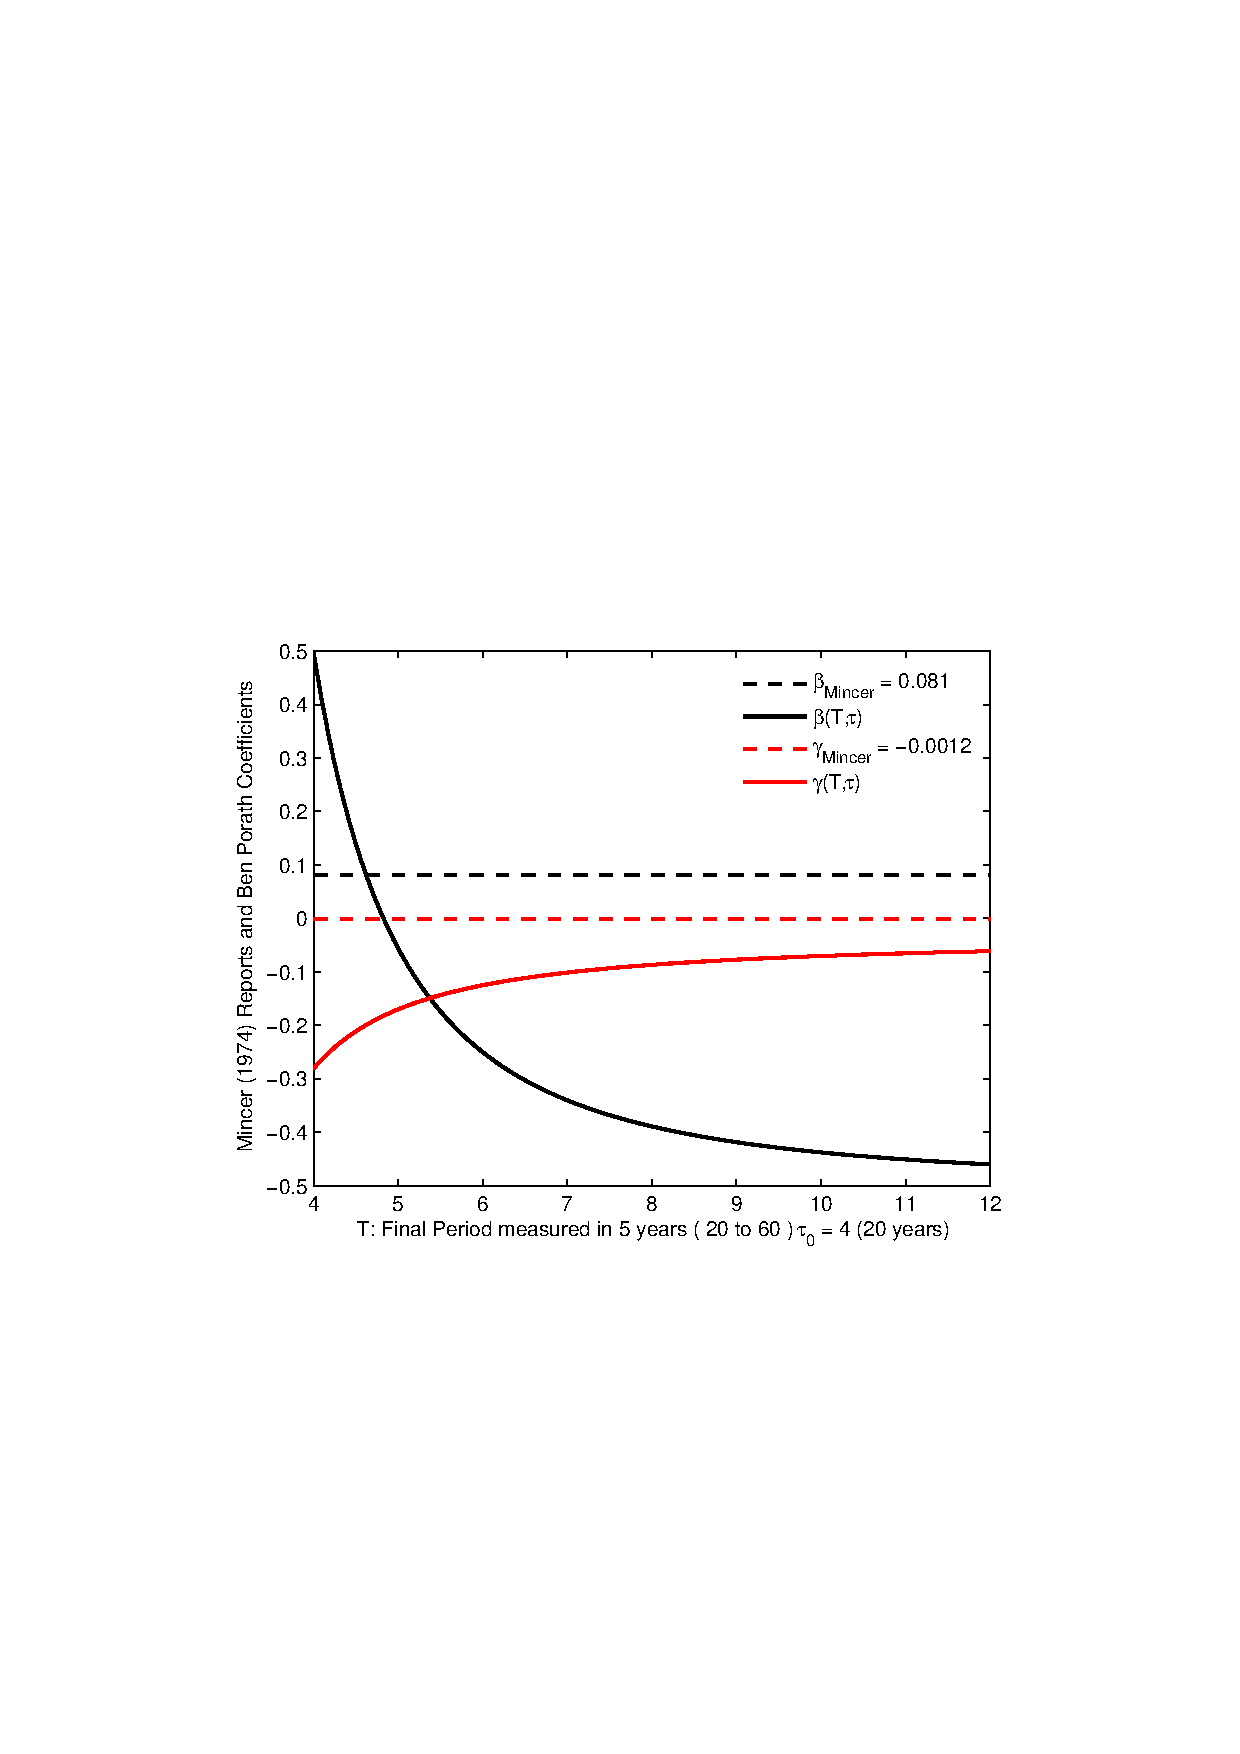
\includegraphics[height=3.0in]{include/BenPorathMincer1.pdf}
%\end{center}
%
%\end{frame}
%
%
%%%%%%%%%%%%%%%%%%%%%%%%%%%%%%%%%%%%%%%%%%%%%%%%%%%%%%%%%%%%%%%%%%%%%%%%%%%%%%%%
%\begin{frame}
%
%\begin{center}
%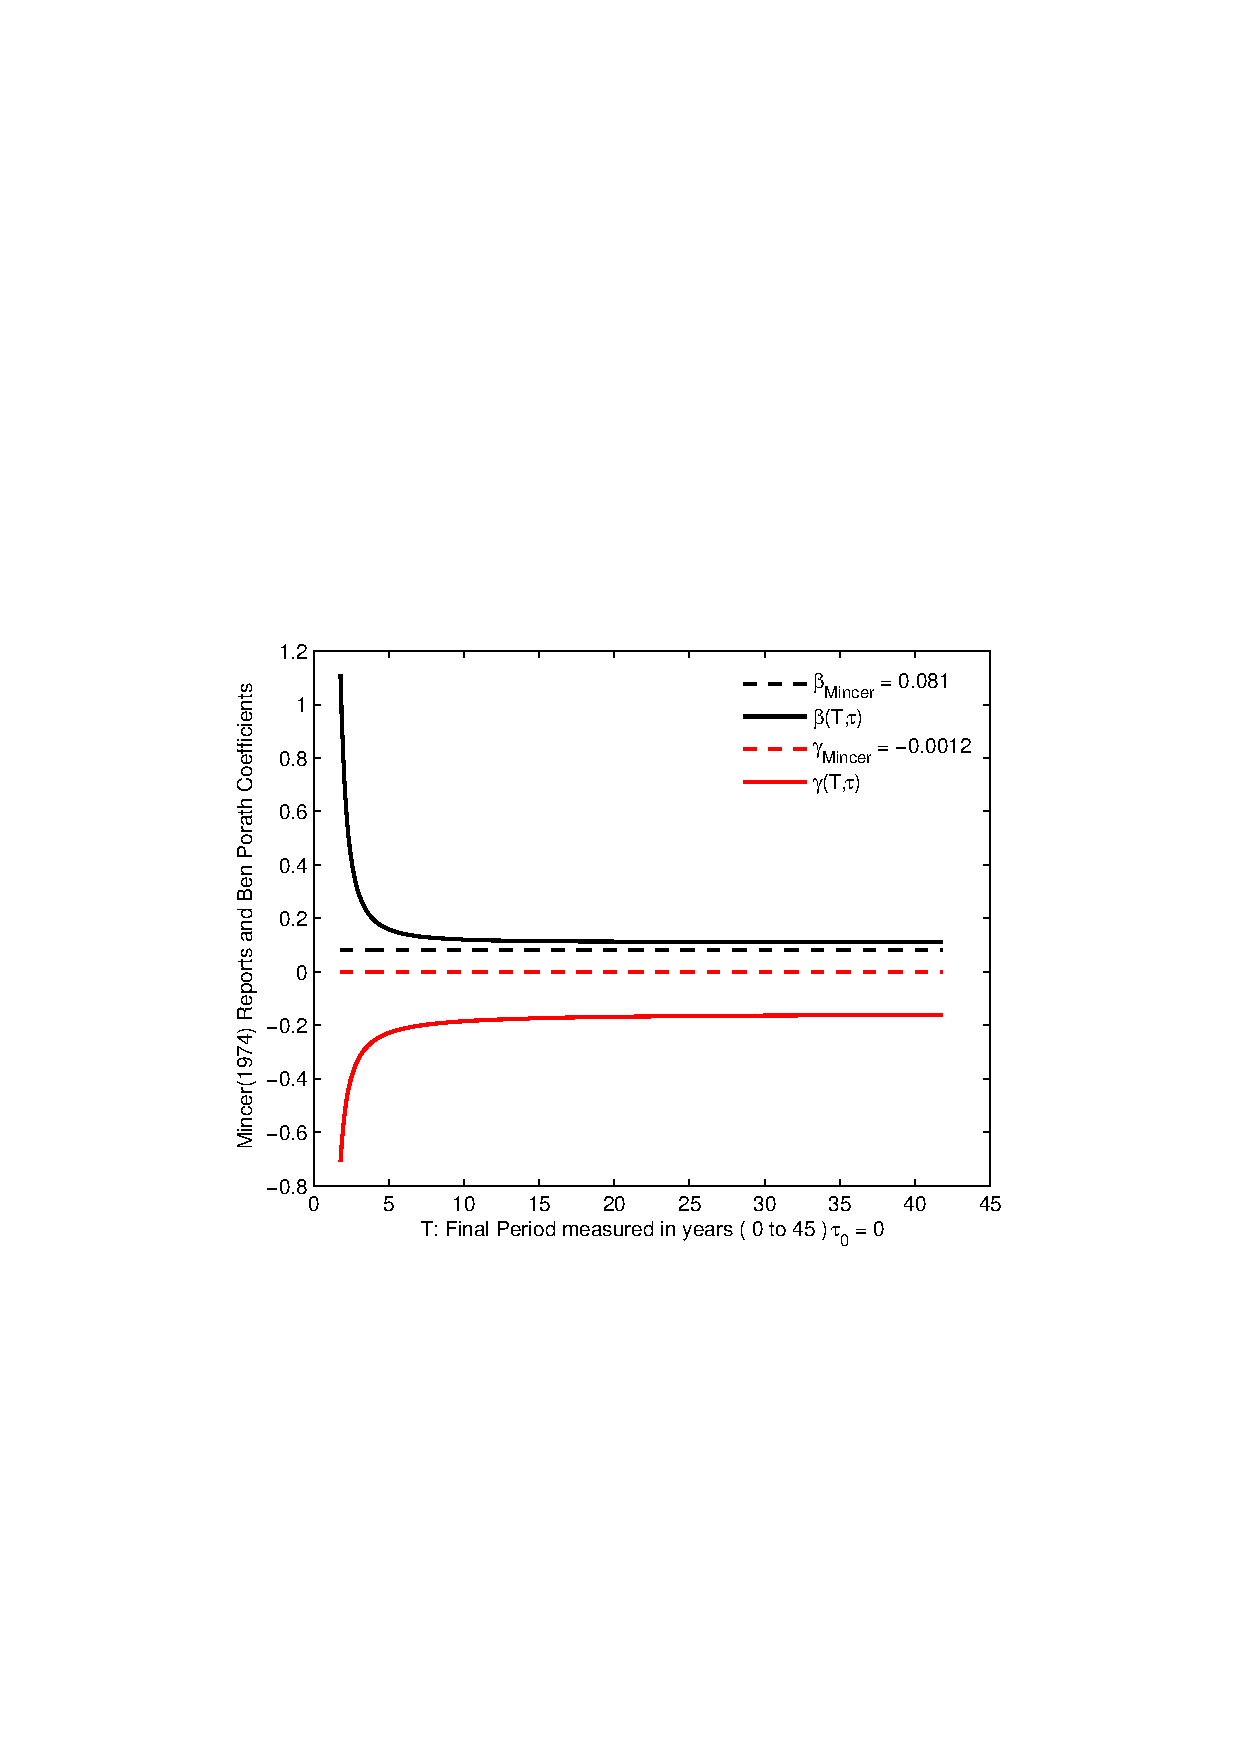
\includegraphics[height=3.0in]{include/BenPorathMincer2.pdf}
%\end{center}
%
%\end{frame}
%
%
%%%%%%%%%%%%%%%%%%%%%%%%%%%%%%%%%%%%%%%%%%%%%%%%%%%%%%%%%%%%%%%%%%%%%%%%%%%%%%%%
%\begin{frame}
%
%\begin{center}
%\includegraphics[height=3.0in]{include/BenPorathMincer3.pdf}
%\end{center}
%
%\end{frame}
%
%
%%%%%%%%%%%%%%%%%%%%%%%%%%%%%%%%%%%%%%%%%%%%%%%%%%%%%%%%%%%%%%%%%%%%%%%%%%%%%%%%
%\begin{frame}
%
%\begin{center}
%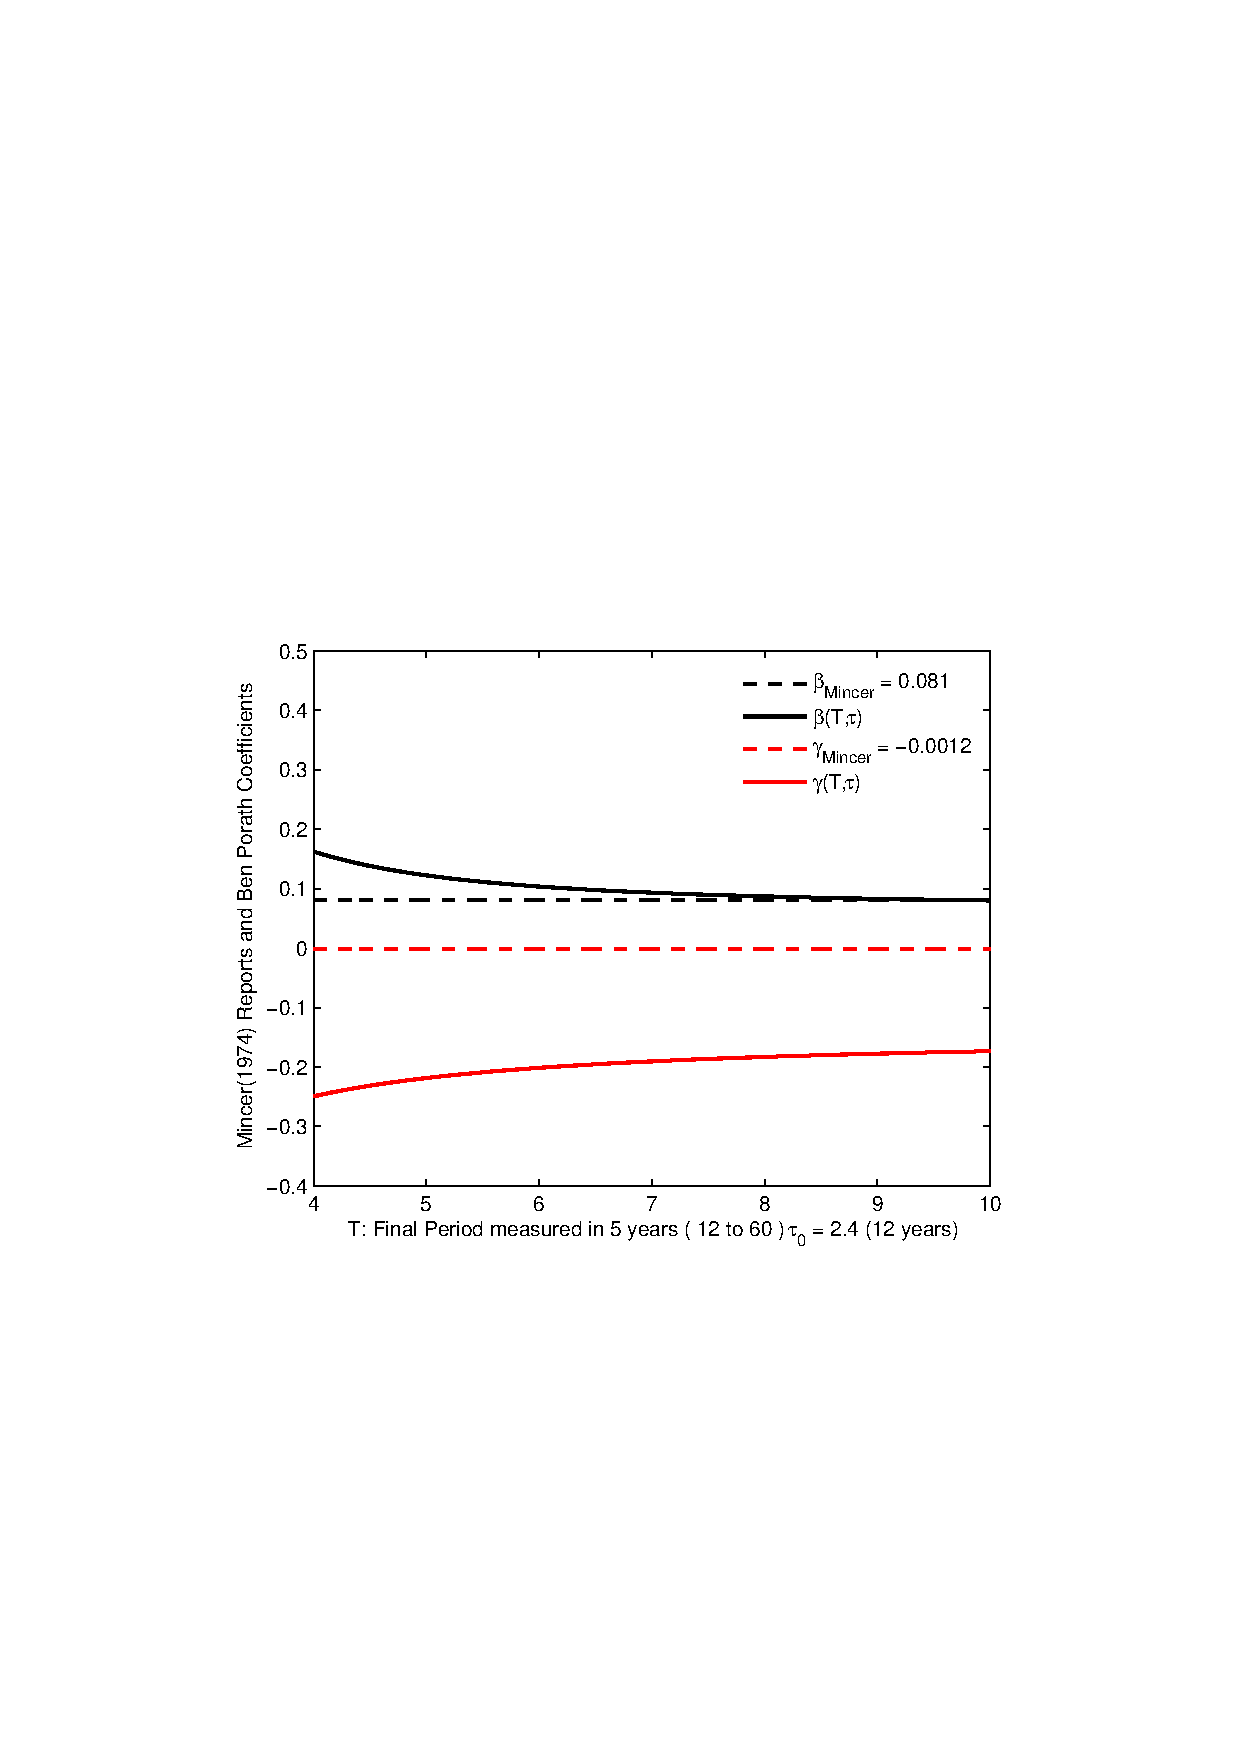
\includegraphics[height=3.0in]{include/BenPorathMincer4.pdf}
%\end{center}
%
%\end{frame}
%
%
%%%%%%%%%%%%%%%%%%%%%%%%%%%%%%%%%%%%%%%%%%%%%%%%%%%%%%%%%%%%%%%%%%%%%%%%%%%%%%%%
%\begin{frame}
%
%\begin{center}
%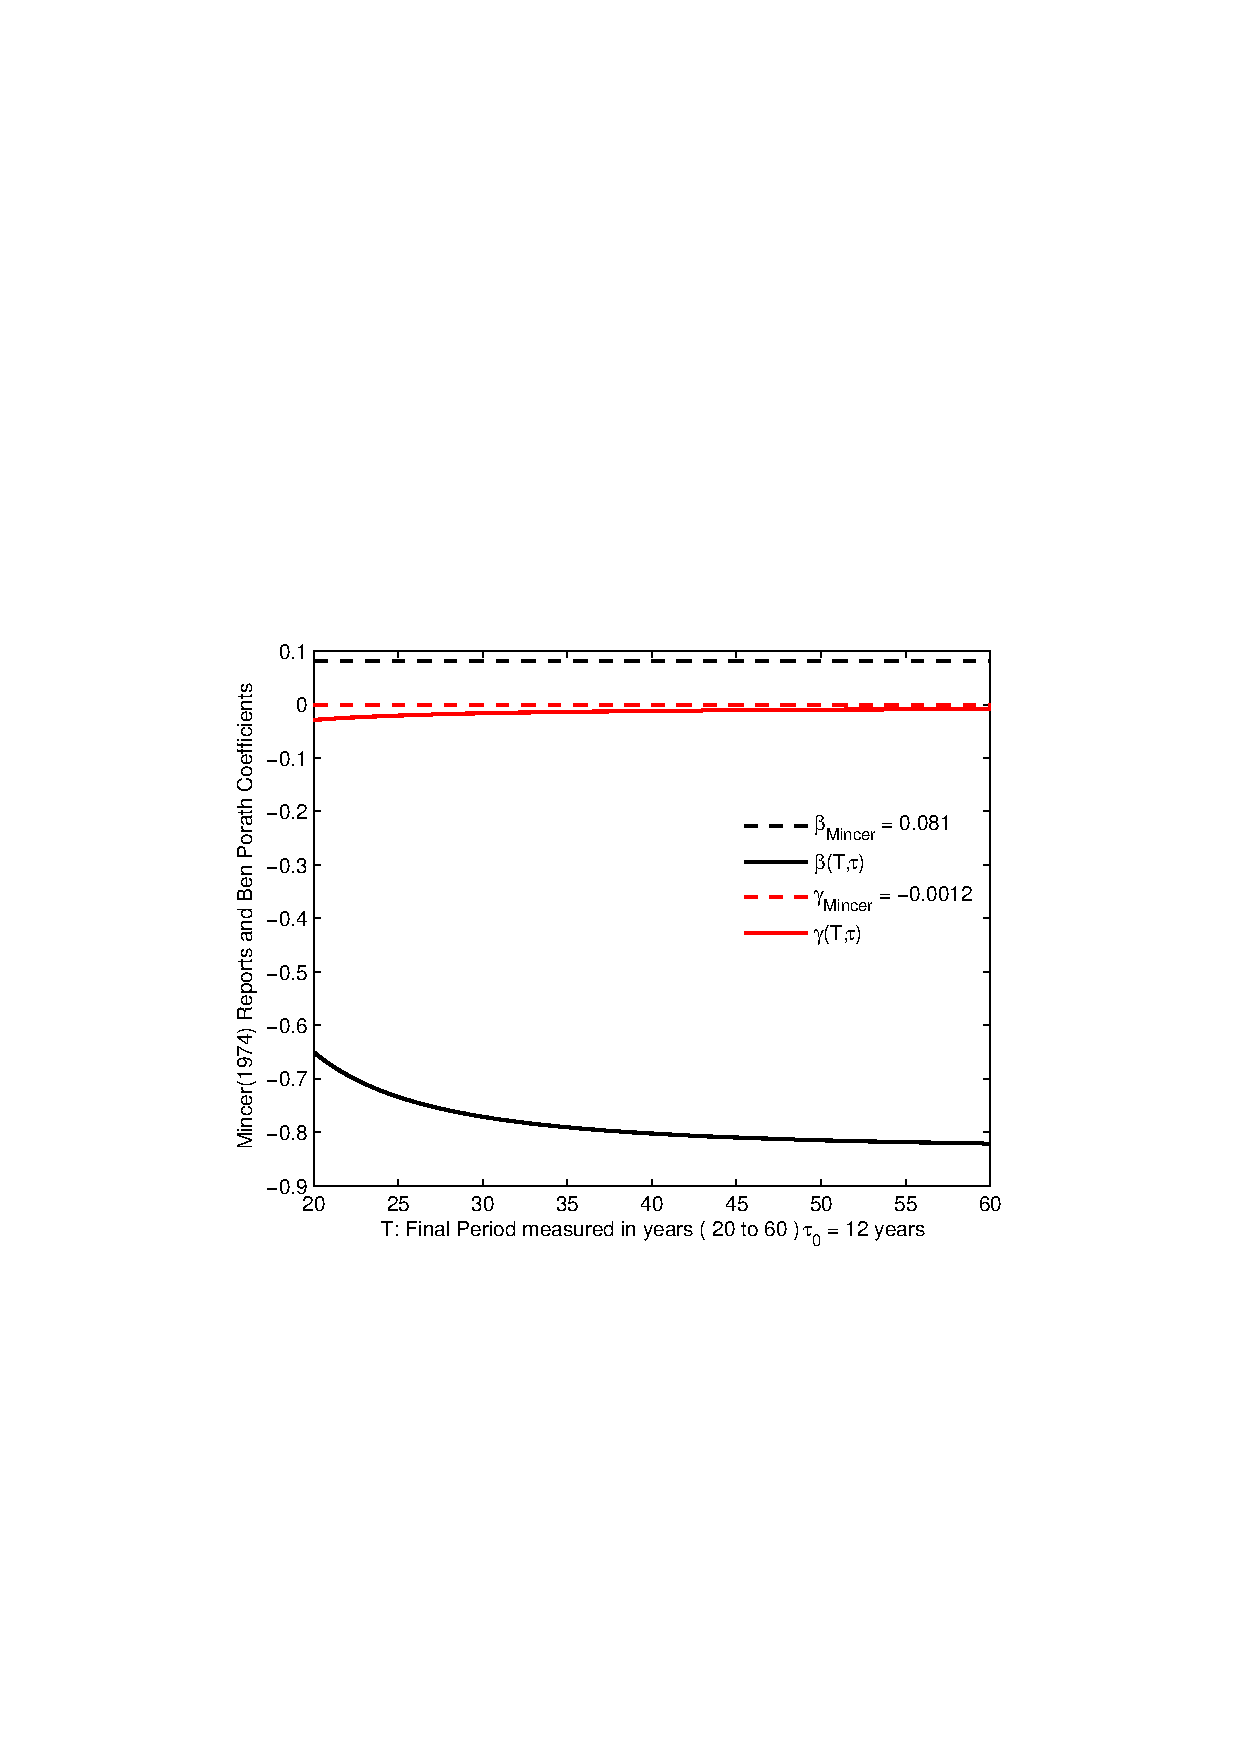
\includegraphics[height=3.0in]{include/BenPorathMincer5.pdf}
%\end{center}
%
%\end{frame}
%
%
%%%%%%%%%%%%%%%%%%%%%%%%%%%%%%%%%%%%%%%%%%%%%%%%%%%%%%%%%%%%%%%%%%%%%%%%%%%%%%%%
%\begin{frame}
%
%\begin{center}
%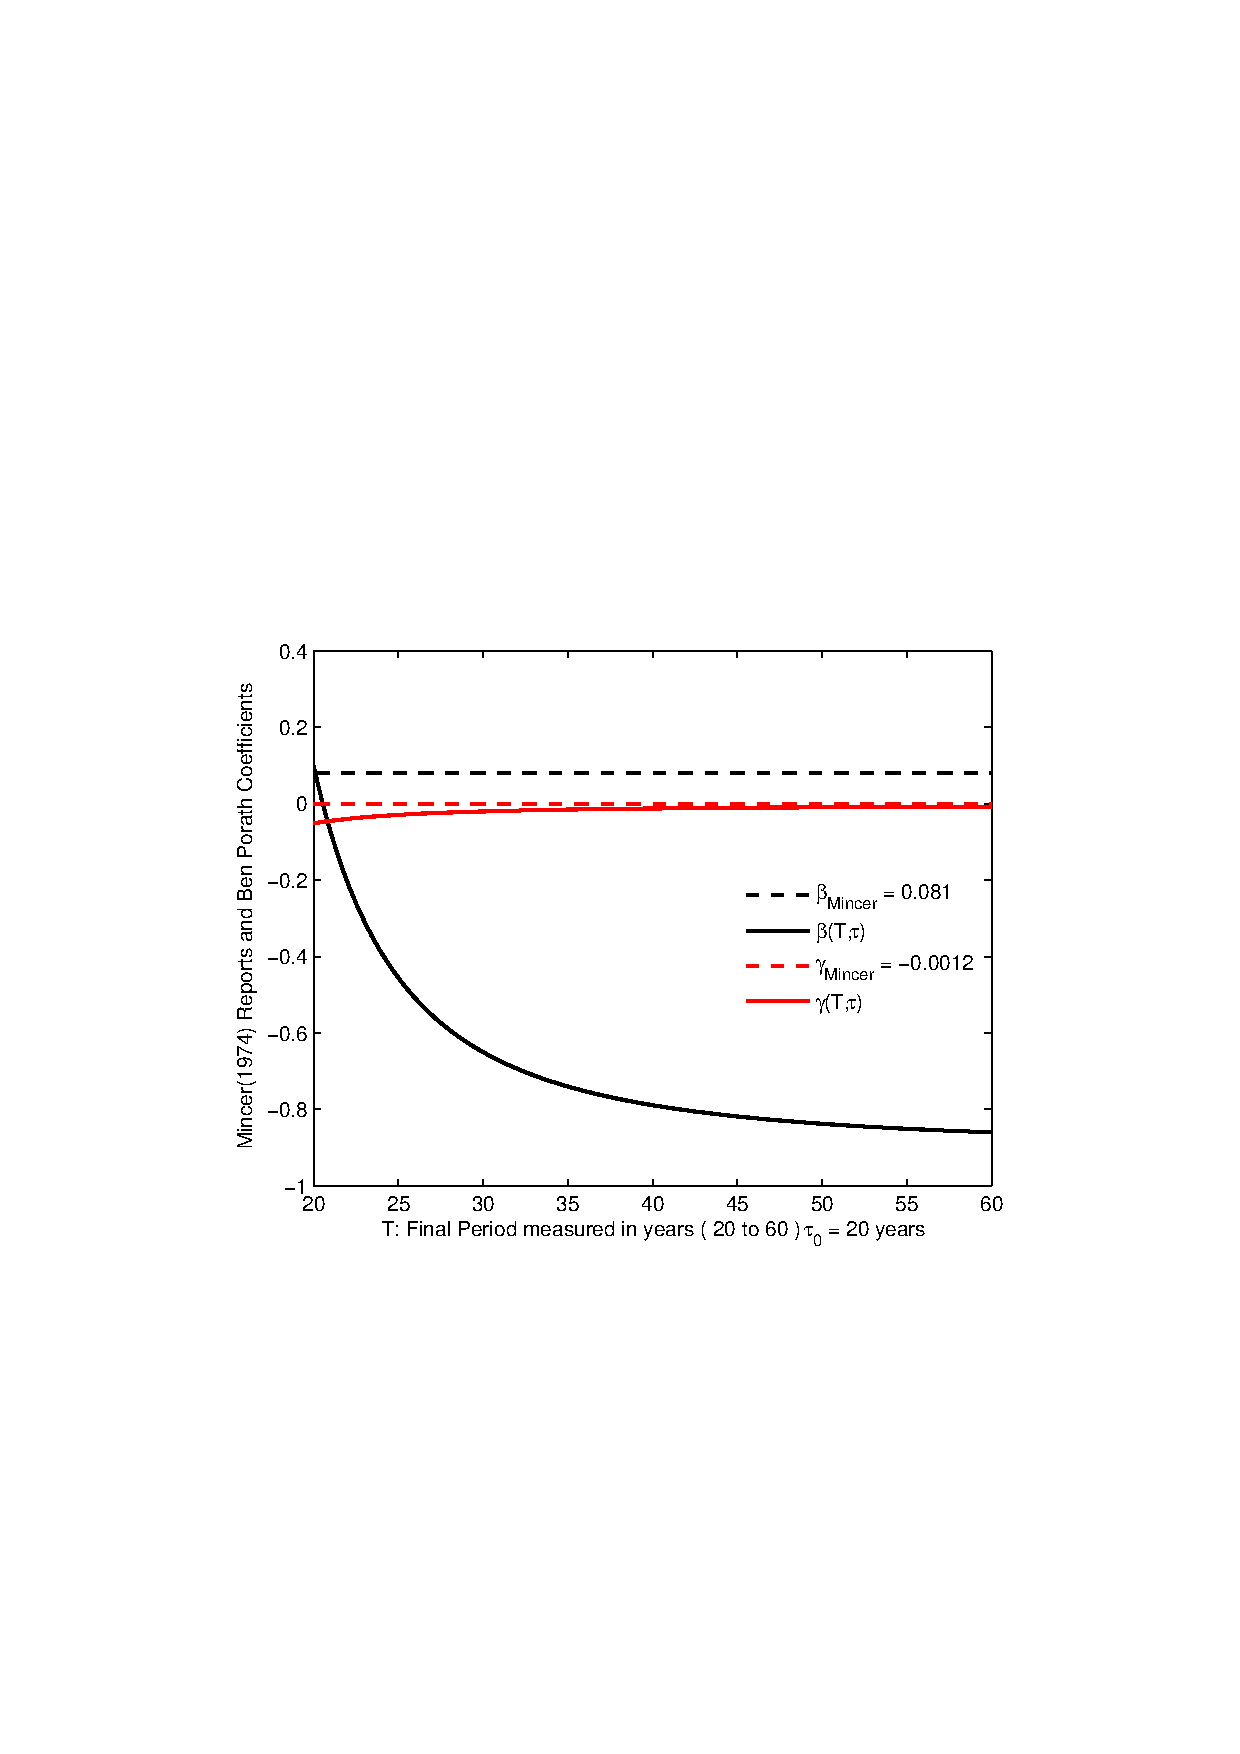
\includegraphics[height=3.0in]{include/BenPorathMincer6.pdf}
%\end{center}
%
%\end{frame}


%%%%%%%%%%%%%%%%%%%%%%%%%%%%%%%%%%%%%%%%%%%%%%%%%%%%%%%%%%%%%%%%%%%%%%%%%%%%%%%
\begin{frame}
\frametitle{\textbf{Conclusion}}

\small
\begin{itemize}
\item
There may be no economic content in Mincer's ``rate of
return'' on post-school investment.\\[5mm]

\item
All of the economic content is in the intercept term.\\[5mm]

\item
Note, however, holding experience constant, there should be no effect of
schooling on the earnings function.\\[5mm]

\item Mincer finds an effect. This would seem to argue against the Ben-Porath
model.\\[5mm]

\item
Not necessarily. Look at equation
\begin{equation*}
    t^{*} = \frac{1}{r} - \frac{1}{2}\,\frac{H^{1/2}_{0}}{A}
    \quad\text{for }\alpha = 1/2 \text{ and } T \text{ ``big.''}
\end{equation*}
\end{itemize}

\end{frame}


%%%%%%%%%%%%%%%%%%%%%%%%%%%%%%%%%%%%%%%%%%%%%%%%%%%%%%%%%%%%%%%%%%%%%%%%%%%%%%%
\begin{frame}
\begin{itemize}
\item Suppose $A$ is randomly distributed in the population.\\[5mm]
\item Then, we have that if $H_0$ is distributed independently of $A$, the coefficient on $t^{*}$ (length of schooling) is
\begin{equation*}
    E\left[
        \left( -\frac{1}{2}\,\frac{H^{1/2}_{0}}{A}\right)\left(2 \ln A\right)
    \right] > 0\text{.}
\end{equation*}\ \\[4mm]
\item Thus, the coefficient on schooling is
\begin{equation*}
    -E\left( H_{0}^{1/2}\right)E\left(\frac{\ln A}{A}\right) \text{.}
\end{equation*}
\end{itemize}
\end{frame}


%%%%%%%%%%%%%%%%%%%%%%%%%%%%%%%%%%%%%%%%%%%%%%%%%%%%%%%%%%%%%%%%%%%%%%%%%%%%%%%
\begin{frame}

If $A$ is Pareto;
\begin{equation*}
    F(A) = \left( \frac{\alpha}{A_0}\right)\left(
    \frac{A_0}{A}\right)^{\alpha+1},
    \quad A_0>0,\,\alpha>0.
\end{equation*}
Integrate by parts to reach
\begin{eqnarray*}
    E\left( \frac{\ln A}{A}\right)
    &=&
    - \frac{(A_0)^{\alpha+1}\alpha}{A_0}(\ln A_0)\,A_0^{-(\alpha+1)} - \frac{1}{\alpha+1}\\
    &=&
    - \frac{\alpha\ln A_0}{A_0} - \frac{1}{\alpha+1}\\
\end{eqnarray*}

\end{frame}


%%%%%%%%%%%%%%%%%%%%%%%%%%%%%%%%%%%%%%%%%%%%%%%%%%%%%%%%%%%%%%%%%%%%%%%%%%%%%%%
\begin{frame}

Therefore, the coefficient on schooling is
\begin{equation*}
    E \left(H_0\right)^{1/2}
        \left[\frac{1}{\alpha+1}+\frac{\alpha\ln A_0}{A_0}\right] > 0.
\end{equation*}
Since units of $H_0$ are arbitrary, we are done.\bigskip

Therefore, positive coefficient on schooling solely as a consequence
of \emph{not} including ability measures.

\end{frame}


%%%%%%%%%%%%%%%%%%%%%%%%%%%%%%%%%%%%%%%%%%%%%%%%%%%%%%%%%%%%%%%%%%%%%%%%%%%%%%%
\section[Rate of Return]{Rate of Return to Post-School Investment}


%%%%%%%%%%%%%%%%%%%%%%%%%%%%%%%%%%%%%%%%%%%%%%%%%%%%%%%%%%%%%%%%%%%%%%%%%%%%%%%
\begin{frame}
\small
\begin{center}
    \textbf{\insertsection}
\end{center}

Let $T\rightarrow\infty$. Without post-school investment, person makes
\begin{equation*}
    R\left[\dfrac{\alpha A}{r}\right]^{\frac{1}{1-\alpha}}.
\end{equation*}
Increment in earnings at post-school age $\tau$ is simply
\begin{equation*}
    \underset{\text{ing earnings) at $\tau $}}{
    \underset{\text{Earnings (above school-}}{
    ~~~~
    \underbrace{
        RA\left[\dfrac{\alpha A}{r}\right]^{\frac{1}{1-\alpha}}\tau
    }-}}
    \underset{\text{Costs}}{
    \underbrace{
        R\left[\dfrac{\alpha A}{r}\right]^{\frac{1}{1-\alpha}}
    }}.
\end{equation*}

\end{frame}


%%%%%%%%%%%%%%%%%%%%%%%%%%%%%%%%%%%%%%%%%%%%%%%%%%%%%%%%%%%%%%%%%%%%%%%%%%%%%%%
\begin{frame}
\begin{itemize}
\item $\phi$ is that rate that equates returns and costs. Thus, solve for~$\phi$.
\begin{equation*}
    \int\limits_{0}^{\infty}
        e^{-\phi \tau}
        \left[
            RA\left[\dfrac{\alpha A}{r}\right]^{\frac{1}{1-\alpha}}\tau
            -
            R\left[\dfrac{\alpha A}{r}\right]^{\frac{1}{1-\alpha}}
        \right]\,d\tau = 0
\end{equation*}\ \\[3mm]
\item Use the Laplace transform.\\[5mm]
\item Then
\begin{gather*}
    \frac{1}{\phi^2}\,RA\left[\dfrac{\alpha A}{r}\right]^{\frac{\alpha}{1-\alpha}}
    -
    \frac{1}{\phi}\,R\left[\dfrac{\alpha A}{r}\right]^{\frac{1}{1-\alpha}}
    = 0\\
    \phi = \frac{r}{\alpha} \text{.}
\end{gather*}
\end{itemize}
\end{frame}

\begin{frame}
\begin{itemize}
\item Therefore the rate of return to post-schooling investment is $r/\alpha$.\\[9mm]
\item Smaller $\alpha$, higher $\phi$.\\[9mm]
\item Thus, the lower the productivity (i.e., $\alpha$), the higher $\phi$.
\end{itemize}
\end{frame}


%%%%%%%%%%%%%%%%%%%%%%%%%%%%%%%%%%%%%%%%%%%%%%%%%%%%%%%%%%%%%%%%%%%%%%%%%%%%%%%
\begin{frame}
\begin{center}
    \textbf{Rate of Return to Schooling (Holding Post-School Investment Fixed)}
\end{center}

Person without schooling can earn $RH_0$. With schooling can earn
$RA\left[\frac{\alpha A}{r}\right]^{\frac{\alpha}{1-\alpha}}$. (Assuming no
post school investment.)\bigskip

Recall that (for $T\rightarrow\infty$), optimal schooling is given
by
\begin{equation*}
    t^{*} = \frac{1}{r} - \frac{1}{2}\frac{H_0^{1/2}}{A}.
\end{equation*}
During this period (before $t^{*}$), under our assumptions, there are no
earnings.

\end{frame}


%%%%%%%%%%%%%%%%%%%%%%%%%%%%%%%%%%%%%%%%%%%%%%%%%%%%%%%%%%%%%%%%%%%%%%%%%%%%%%%
\begin{frame}

\footnotesize

Then the rate of return is given by comparing \small
\begin{equation*}
    \int\limits_{t^{*}}^{\infty}
        e^{-\phi t}
        \left[
            R \left(\frac{\alpha A}{r}\right)^{\frac{1}{1-\alpha}}
        \right]\,dt
    \text{ with }
    \int\limits_{0}^{\infty} e^{-\phi t} R H_0\,dt.
\end{equation*}
Solve for $\phi$:
\begin{eqnarray*}
    \left[ \frac{\alpha A}{r}\right]^{\frac{1}{1-\alpha}} e^{-\phi t^{*}}
    &=&
    H_0\\
    \ln \left[ \frac{\alpha A}{r}\right]^{\frac{1}{1-\alpha}} - \phi t^{*}
    &=&
    \ln H_0\\
    \phi
    =
    \frac{\ln \left[ \frac{\alpha A}{r}\right]^{\frac{1}{1-\alpha}} - \ln H_0}{t^{*}}
    &=&
    \frac{\ln \left[ \frac{\alpha A}{r}\right]^{\frac{1}{1-\alpha}} - \ln H_0}
        {\frac{1}{r}-\frac{1}{2}\frac{H_0^{1/2}}{A}}
\end{eqnarray*}

Has no simple relationship to the rate of return to investment.
\end{frame}


%%%%%%%%%%%%%%%%%%%%%%%%%%%%%%%%%%%%%%%%%%%%%%%%%%%%%%%%%%%%%%%%%%%%%%%%%%%%%%%
\section[Growth]{Growth of Earnings}


%%%%%%%%%%%%%%%%%%%%%%%%%%%%%%%%%%%%%%%%%%%%%%%%%%%%%%%%%%%%%%%%%%%%%%%%%%%%%%%
\begin{frame}
\begin{center}
    \textbf{\insertsection}
\end{center}
\end{frame}


%%%%%%%%%%%%%%%%%%%%%%%%%%%%%%%%%%%%%%%%%%%%%%%%%%%%%%%%%%%%%%%%%%%%%%%%%%%%%%%
\begin{frame}

\begin{itemize}
\item
Keep time argument implicit unless being explicit helps.\\[3mm]

\item
$E$, $H$, $IH$ all depend on $t$.\\[3mm]

\item
Growth of earnings:
\begin{align*}
\dot{E} & =f(IH)-(\dot{IH})\\[3mm]
\frac{\partial \dot{E}}{\partial r} & =\ \text{\large ?}
\end{align*}\ \\[3mm]
\item FOC:
\begin{align*}
g(t)\,f'(IH) & =1\\[3mm]
g(t) & =\frac{1-e^{r(t-T)}}{r}
\end{align*}
\end{itemize}
\end{frame}


%%%%%%%%%%%%%%%%%%%%%%%%%%%%%%%%%%%%%%%%%%%%%%%%%%%%%%%%%%%%%%%%%%%%%%%%%%%%%%%
\begin{frame}

\begin{itemize}
\item
Totally differentiate FOC with respect to $t$:
\begin{align*}
\dot{g}f'(IH)+gf''(IH)(\dot{IH}) & =0\\[3mm]
-\left( \frac{\dot{g}}{g}\frac{f'}{f''}\right) & =(\dot{IH})
\end{align*}\ \\[3mm]
\item First note that
\begin{equation*}
\frac{\partial \dot{E}}{\partial r}=f'\left( \frac{\partial
IH}{\partial r}\right) -\frac{\partial }{\partial r}\left[
(\dot{IH})\right] \text{.}
\end{equation*}
\end{itemize}

\end{frame}


%%%%%%%%%%%%%%%%%%%%%%%%%%%%%%%%%%%%%%%%%%%%%%%%%%%%%%%%%%%%%%%%%%%%%%%%%%%%%%%
\begin{frame}

\begin{itemize}
\item
Now observe further that
\begin{equation*}
\frac{\partial (IH)}{\partial r}<0\text{.}
\end{equation*}\ \\[3mm]

\item
Thus the first term is negative.\\[5mm]

\item
Observe that we can show that
\begin{equation*}
\frac{\partial (\dot{IH})}{\partial r}>0
\end{equation*}
if concavity on earnings is satisfied ($\ddot{E}<0$).
\end{itemize}
\end{frame}


%%%%%%%%%%%%%%%%%%%%%%%%%%%%%%%%%%%%%%%%%%%%%%%%%%%%%%%%%%%%%%%%%%%%%%%%%%%%%%%
\begin{frame}

\begin{itemize}
\item
Intuition: the time rate of decrease in $IH$ is slowed down ($r
\uparrow \
\Rightarrow IH \downarrow$\,;\ \,the function is ``less concave'').\\[12mm]

\item
If we can establish this, we know that the contribution of the
second term is negative and
\begin{equation*}
\frac{\partial \dot{E}}{\partial r}<0\text{.}
\end{equation*}
\end{itemize}

\end{frame}


%%%%%%%%%%%%%%%%%%%%%%%%%%%%%%%%%%%%%%%%%%%%%%%%%%%%%%%%%%%%%%%%%%%%%%%%%%%%%%%
\begin{frame}

\begin{itemize}
\item
To show this, observe that
\begin{equation*}
\frac{\partial [\dot{IH}]}{\partial r}=\left[
-\frac{\dot{g}}{g}\right] \left[ 1-\frac{f'f'''}{(f'')^2}\right]
\frac{\partial (IH)}{\partial r}+\left( \frac{f'}{f''}\right)
\frac{\partial }{\partial r}\left[ -\frac{\dot{g}}{g}\right]
\text{.}
\end{equation*}\ \\[7mm]

\item
From the earlier notes, concavity of earnings function in experience $(\ddot{E}<0)$
\begin{equation*}
\left[ 1-\frac{f'f'''}{(f'')^2}\right] <0\text{.}
\end{equation*}
\end{itemize}
\end{frame}


%%%%%%%%%%%%%%%%%%%%%%%%%%%%%%%%%%%%%%%%%%%%%%%%%%%%%%%%%%%%%%%%%%%%%%%%%%%%%%%
\begin{frame}

\begin{itemize}
\item The first term is positive, since $\dot{g}<0$ and
\begin{equation*}
\frac{\partial (IH)}{\partial r}<0\text{.}
\end{equation*}\ \\[9mm]
\item To investigate the second term, we determine that
\begin{equation*}
\dot{g}=rg-1\,\text{,}\hspace{8mm}
\frac{\dot{g}}{g}=r-\frac{1}{g}\,\text{,}\hspace{8mm}
-\frac{\dot{g}}{g}=\frac{1}{g}-r\,\text{.}
\end{equation*}
\end{itemize}

\end{frame}


%%%%%%%%%%%%%%%%%%%%%%%%%%%%%%%%%%%%%%%%%%%%%%%%%%%%%%%%%%%%%%%%%%%%%%%%%%%%%%%
\begin{frame}

\begin{itemize}
\item Now,
\begin{equation*}
\frac{\partial }{\partial r}\left[ -\frac{\dot{g}}{g}\right]
=-\frac{1}{g^2}\frac{\partial g}{\partial r}-1\text{.}
\end{equation*}\ \\[11mm]
\item This term is negative. Why?
\end{itemize}

\end{frame}


%%%%%%%%%%%%%%%%%%%%%%%%%%%%%%%%%%%%%%%%%%%%%%%%%%%%%%%%%%%%%%%%%%%%%%%%%%%%%%%
\begin{frame}

\begin{itemize}
\item \ \\[-12mm]
\begin{align*}
\frac{\partial g}{\partial r} & =\frac{-(t-T)e^{r(t-T)}}{r}-\frac{1-e^{r(t-T)}}{r^2}\\[3mm]
& =\frac{1}{r^2}\left[ e^{r(t-T)}\left( 1-r(t-T)\right) -1\right]
\end{align*}\ \\[3mm]
\item Now observe that
\begin{equation*}
e^{r(T-t)}>1+r(T-t)\hspace{9mm}\text{for }T\geq t\,\text{.}
\end{equation*}\ \\[3mm]
\item Thus
\begin{equation*}
\frac{\partial g}{\partial r}<0\text{.}
\end{equation*}
\end{itemize}

\end{frame}


%%%%%%%%%%%%%%%%%%%%%%%%%%%%%%%%%%%%%%%%%%%%%%%%%%%%%%%%%%%%%%%%%%%%%%%%%%%%%%%
\begin{frame}

\begin{itemize}
\item Consider next that
\begin{align*}
&\frac{-\partial g}{g^2\partial r}-1=\frac{1}{r^2}\left[ \frac{1-e^{r(t-T)}\left( 1-r(t-T)\right)}{g^2}\right] -1\\[3mm]
&\hspace{3mm}=\frac{1}{g^2r^2}\left[ 1-e^{r(t-T)}\left(1-r(t-T)\right) -\left(1-e^{r(t-T)}\right) ^2\right] \\[3mm]
&\hspace{3mm}=\frac{1}{(rg)^2}\left[ 1-e^{r(t-T)}\left(1-r(t-T)\right) -1+2e^{r(t-T)}-e^{2r(t-T)}\right] \\[3mm]
&\hspace{3mm}=\frac{1}{(rg)^2}\left[ e^{r(t-T)}\right] \left[
1+r(t-T)-e^{r(t-T)}\right] \text{.}
\end{align*}
\end{itemize}

\end{frame}


%%%%%%%%%%%%%%%%%%%%%%%%%%%%%%%%%%%%%%%%%%%%%%%%%%%%%%%%%%%%%%%%%%%%%%%%%%%%%%%
\begin{frame}

\begin{itemize}
\item This expression is clearly negative.\\[3mm]

\item
Set $x\equiv T-t$:\\[3mm]
\end{itemize}
\begin{enumerate}[(1)]
\item \ \\[-10mm]
\begin{equation*}
1-rx-e^{-rx}=0\hspace{6mm}\text{when }x=0\text{.}
\end{equation*}\ \\[5mm]
\item \ \\[-10mm]
\begin{equation*}
\frac{\partial }{\partial x}\left( 1-rx-e^{-rx}\right)
=-r+re^{-rx}<0\text{.}
\end{equation*}
\end{enumerate}\ \\[6mm]
\begin{itemize}
\item Thus from concavity ($f''<0$),
\begin{equation*}
\left( \frac{f'}{f''}\right) \frac{\partial }{\partial r}\left[
-\frac{\dot{g}}{g}\right] >0\text{.}
\end{equation*}\ \\[4mm]
\item Now the proposition is proved for $\sigma =0$ with $\ddot{E}<0$ everywhere. {\itshape Q.E.D.}
\end{itemize}
\end{frame}


%%%%%%%%%%%%%%%%%%%%%%%%%%%%%%%%%%%%%%%%%%%%%%%%%%%%%%%%%%%%%%%%%%%%%%%%%%%%%%%
\begin{frame}

\begin{center}
\includegraphics[width=4.75in]{include/fig-earnings-growth}
\end{center}

\end{frame}


%%%%%%%%%%%%%%%%%%%%%%%%%%%%%%%%%%%%%%%%%%%%%%%%%%%%%%%%%%%%%%%%%%%%%%%%%%%%%%%
\section[Appendix]{Appendix: Haley-Rosen}


%%%%%%%%%%%%%%%%%%%%%%%%%%%%%%%%%%%%%%%%%%%%%%%%%%%%%%%%%%%%%%%%%%%%%%%%%%%%%%%
\begin{frame}

\textbf{\insertsection:} Let $\alpha =1/2$.
\begin{equation*}
    E(\tau )
    =
    RH(t^{*})+R\int\limits_{0}^{\tau }A\left( \dfrac{1}{2}
        \dfrac{g(t^{*}+\ell )A}{R}\right) \,d\ell
    -R\left[ \dfrac{1}{2}\dfrac{g(\tau +t^{*})A}{R}\right] ^{2}.
\end{equation*}
This can be written as a simple autoregression in earnings: {\small
\begin{eqnarray*}
    \dot{E}(\tau )
    &=&
    R\left[
        A\left( \frac{1}{2}\frac{g(t^{*}+\tau )A}{R}\right)
        -2R\left[ \frac{1}{2}\frac{g(\tau +t^{*})A}{R}\right] \frac{A}{2R}
        \dot{g}(\tau +t^{*})
    \right] \\
    &=&
    \frac{1}{2}A^{2}[g(t^{*}+\tau )(R-\dot{g}(t^{*}+\tau )].\\\\
    \dot{g}
    &=&
    rg-R
\end{eqnarray*}
}
\end{frame}


%%%%%%%%%%%%%%%%%%%%%%%%%%%%%%%%%%%%%%%%%%%%%%%%%%%%%%%%%%%%%%%%%%%%%%%%%%%%%%%
\begin{frame}
Thus
\begin{eqnarray*}
    \dot{E}(\tau )
    &=&
    \frac{A^2}{2R}\left[g(t^{*}+\tau)
    \left(R-\dot{g}(t^{*}+\tau)\right)\right]\\\\\\
\dot{g} &=&rg-R \\
\ddot{g} &=&r\dot{g}.
\end{eqnarray*}
\end{frame}


%%%%%%%%%%%%%%%%%%%%%%%%%%%%%%%%%%%%%%%%%%%%%%%%%%%%%%%%%%%%%%%%%%%%%%%%%%%%%%%
\begin{frame}

\textbf{Haley-Rosen:} $\alpha = \beta = 1/2$ {\small
\begin{eqnarray*}
    E(\tau )
    &=&
    RH(t^{*})+R\int\limits_{0}^{\tau }A\left( \frac{1}{2}
    \frac{g(t^{*}+\ell )A}{R}\right) \,d\ell
    -R\left[ \frac{A}{2}\frac{g(\tau +t^{*})}{R}\right]^2\\\\
    \dot{E}(\tau )
    &=&\frac{A^{2}}{2}g(\tau +\tau ^{*})
        -2R\left[ \frac{A}{2}\frac{g(\tau+t^{*})}{R}\right]
        \left[ \frac{A}{2R}\dot{g}\right] \\
    &=&\frac{A^{2}}{2}g(\tau +t^{*})-\frac{1}{2}\frac{A^{2}}{R}g\dot{g} \\
    &=&\frac{1}{2}A^{2}g\left[ 1-\frac{\dot{g}}{R}\right]
        \qquad\text{use: } \dot{g}=rg-R \\
    &=&\frac{1}{2}\frac{A^{2}}{R}g[R-\dot{g}]=\frac{A^{2}}{2R}g[R-rg+R] \\
    &=&\frac{A^{2}}{2R}g[2R-rg]
\end{eqnarray*}
}

\end{frame}


%%%%%%%%%%%%%%%%%%%%%%%%%%%%%%%%%%%%%%%%%%%%%%%%%%%%%%%%%%%%%%%%%%%%%%%%%%%%%%%
\begin{frame}

\begin{eqnarray*}
    \ddot{E}(\tau ) &=&\frac{A^{2}}{2R}[\dot{g}(2R-rg)+g(-r\dot{g})] \\
    &=&\frac{A^{2}}{2R}\dot{g}[2R-2rg]=\frac{A^{2}}{R}\dot{g}(R-rg) \\
    &=&-\frac{A^{2}}{2}(\dot{g})^{2}.
\end{eqnarray*}
Notice that $\dot{E}(\tau )$\ can be written as
\begin{eqnarray*}
    \dot{E}(\tau )
    &=&\frac{A^{2}}{2R}\left( \frac{\dot{g}+R}{r}\right)
        \left(2R-r\frac{(\dot{g}+R)}{r}\right)  \\
    &=&\frac{A^{2}}{2R}\left( \frac{\dot{g}+R}{r}\right) (2R-\dot{g}-R) \\
    &=&\frac{A^{2}}{2R}\left( \frac{\dot{g}+R}{r}\right) (R-\dot{g})
        =\frac{A^{2}}{2Rr}(R^{2}-(\dot{g})^{2}).
\end{eqnarray*}

\end{frame}


%%%%%%%%%%%%%%%%%%%%%%%%%%%%%%%%%%%%%%%%%%%%%%%%%%%%%%%%%%%%%%%%%%%%%%%%%%%%%%%
\begin{frame}

Thus we conclude that
\begin{eqnarray*}
    \dot{E}(\tau)
    &=& \frac{A^{2}}{2Rr}R^{2}
        - \frac{1}{2r}\frac{A^2}{R}(\dot{g})^{2}\\
    &=& \frac{A^{2}}{2Rr}R^{2} + \frac{1}{2r}\ddot{E}
\end{eqnarray*}
 so that
\begin{equation*}
    \ddot{E}(\tau ) - 2r\dot{E}(\tau ) + A^{2}R=0.
\end{equation*}
Integrate once to reach
\begin{equation*}
    \dot{E}(\tau ) - 2rE(\tau ) + A^{2}R\tau + c_{0}=0
\end{equation*}
where $c_0$ is a constant of integration.

\end{frame}


%%%%%%%%%%%%%%%%%%%%%%%%%%%%%%%%%%%%%%%%%%%%%%%%%%%%%%%%%%%%%%%%%%%%%%%%%%%%%%%
\begin{frame}

Then ``reduced equation'' is
\begin{equation*}
    \dot{E}(\tau ) = 2rE(\tau )
\end{equation*}
so that
\begin{equation*}
    E(\tau )
    =
    c_{1} e^{2r\tau },
\end{equation*}
$c_1$ is constant of integration.\bigskip

The general solution is thus:
\begin{equation*}
    E(\tau )
    =
    c_{0} + c_{2}\tau + c_{1}e^{2r\tau}.
\end{equation*}

\end{frame}


%%%%%%%%%%%%%%%%%%%%%%%%%%%%%%%%%%%%%%%%%%%%%%%%%%%%%%%%%%%%%%%%%%%%%%%%%%%%%%%
\begin{frame}

For a period of specialization, $E(0)=0$ so that $c_{1}+c_{0}=0$.
\begin{equation*}
    \dot{E}(\tau ) = 2rc_{1}e^{2r\tau }+c_{2}
\end{equation*}
so that at $\tau =0$,{\footnotesize
\begin{gather*}
    (2r c_{1} e^{2r\tau }+c_{2})
    - 2r[c_{1}e^{2r\tau }+c_{0}+c_{2}\tau ]+A^{2}R\tau +c_{0}=0\text{.}
\end{gather*}
} Thus we conclude that {\footnotesize
\begin{equation*}
c_2 = \frac{A^2R}{2r}
\end{equation*}
}

\end{frame}


%%%%%%%%%%%%%%%%%%%%%%%%%%%%%%%%%%%%%%%%%%%%%%%%%%%%%%%%%%%%%%%%%%%%%%%%%%%%%%%
\begin{frame}

To this point, the equation looks like
\begin{equation*}
    E(\tau )=c_{0}(1-e^{2r\tau })+\dfrac{A^{2}R}{2r}\tau.
\end{equation*}
Now there is no investment at the end of life.
\begin{equation*}
    \dot{E}(\tau )=0.
\end{equation*}
Thus
\begin{equation*}
    \dot{E}(T)=0=-2rc_{0}e^{2rT}+\dfrac{A^{2}R}{2r}
\end{equation*}
so $c_{0}=\dfrac{A^{2}R}{(2r)^{2}}e^{-2rT}$. Thus
\begin{equation*}
    E(\tau )=\dfrac{A^{2}R}{(2r)^{2}}e^{-2rT}(1-e^{2r\tau })
        +\dfrac{A^{2}R}{2r}\tau.
\end{equation*}

\end{frame}




\end{document}
